\documentclass[a4paper,12pt]{article}
\usepackage[utf8]{inputenc}

% Variables
%Variablen welche innerhalb der gesamten Arbeit zur Verfügung stehen sollen
\newcommand{\titleDocument}{Bachelor Thesis}
\newcommand{\subjectDocument}{in Computational Linguistics}


% Embed PNG graphics
\usepackage{graphicx}
% Figures next to each other
\usepackage{caption}
\usepackage{subcaption}
% English syllabification
\usepackage[english]{babel}
% West European encoding
\usepackage[T1]{fontenc}
% Smoother font
\usepackage{lmodern}
% Enable floating picture environments
%\usepackage{floatflt}
% Enable multi-page tables
\usepackage{longtable}
% Pretty state of the art tables
\usepackage{tabularx,booktabs}
\newcolumntype{C}{>{\centering\arraybackslash}X} % centered version of "X" type
% Set page margins
\usepackage{geometry}
\geometry{left=3.5cm, right=2cm, top=2.5cm, bottom=2cm}
% Boxes in text
\usepackage{fancybox}
% Appropriately 'syllabify' URLs
\usepackage[hyphens,obeyspaces,spaces]{url}
% Enable colored text
\usepackage{color}
% Import math symbols -- mathtools works better for this document
%\usepackage{amssymb}
% Allow writing above/below arrows + math symbols
\usepackage{mathtools}
% Compile graphics in document with tikz.
\usepackage{tikz}
\usetikzlibrary{positioning, fit, arrows.meta, shapes, automata}
% Heading on each page (centered)
%\pagestyle{headings}
% Easily position graphics
\usepackage[export]{adjustbox}

% Enable hyperlinked Table of Contents in the PDF
\usepackage[bookmarksnumbered,pdftitle={\titleDocument},hyperfootnotes=false]{hyperref}
% Hyperlink settings
%\hypersetup{colorlinks, citecolor=red, linkcolor=blue, urlcolor=black}
%\hypersetup{colorlinks, citecolor=black, linkcolor= black, urlcolor=black}
% Cleaner headings
\usepackage{fancyhdr}
\pagestyle{fancy}
\fancyhf{} % Clean all headings/footings.
%\fancyhead[L]{\nouppercase{\leftmark}} % Left-bound heading
\fancyhead[C]{} % Centered heading
%\fancyhead[R]{\thepage} % Right-bound heading
\renewcommand{\headrulewidth}{0.4pt} %obere Trennlinie
\setlength{\headheight}{15pt}
\fancyfoot[C]{\thepage} % Include page number
%\renewcommand{\footrulewidth}{0.4pt} % Separate line at bottom of the page, does not look good imo
% Citation form: Name (Year)
\usepackage{natbib}
% Set spacing between lines - if requested
\usepackage{setspace}
% Enable captioning non-float environments
\usepackage{capt-of}
% Enable indexing - \see, \seealso, \index...
\usepackage{makeidx}
% Create index if makeidx is enabled
\makeindex
% Enable listings for code/pseudocode
%\usepackage{listings}
%\lstset{numbers=left, numberstyle=\tiny, numbersep=5pt, keywordstyle=\color{black}\bfseries, stringstyle=\ttfamily,showstringspaces=false,basicstyle=\footnotesize,captionpos=b}
%\lstset{language=python}

% List of Abbreviations -- does not work so far
\usepackage[english]{nomencl}
\let\abbrev\nomenclature
% Create index of abbreviations
\makenomenclature
% Abkürzungsverzeichnis LiveTex Version
% Title
\renewcommand{\nomname}{List of Abbreviations}
% Space between abbreviation and explanation
\setlength{\nomlabelwidth}{.25\textwidth}
% Fill space with dots
\renewcommand{\nomlabel}[1]{#1 \dotfill}
% Space between abbreviations
\setlength{\nomitemsep}{-\parsep}
\makeglossary

% Enable linguistic glossing and more. Always load last!!!
\usepackage{gb4e}
\noautomath % gb4e redefines underscores - this suppresses the redefinition

% Suppress orphans
%\clubpenalty = 10000
% Suppress widows
%\widowpenalty = 10000
%\displaywidowpenalty = 10000

\begin{document}
% Begin with empty page for print version
%\thispagestyle{empty}
%\mbox{}
%\newpage

% TITLE PAGE %
\thispagestyle{empty}


\begin{figure}[t]
	\centering
	\includegraphics[width=0.3\textwidth]{fig/humanlogo}
\end{figure}


\begin{verbatim}


\end{verbatim}

\begin{center}
\Large{University of Potsdam}\\
%\Large{- Campus <Name> -}\\
\end{center}


\begin{center}
\Large{Faculty of Human Sciences}
\end{center}
\begin{verbatim}




\end{verbatim}
\begin{center}
\doublespacing
\textbf{\LARGE{\titleDocument}}\\
\singlespacing
\begin{verbatim}

\end{verbatim}
\textbf{{~\subjectDocument~}}
\end{center}
\begin{verbatim}

\end{verbatim}
\begin{center}

\end{center}
\begin{verbatim}

\end{verbatim}
\begin{center}
\textbf{Submitted in Fulfillment of the Requirements for the Degree of \\ Bachelor of Science}
\end{center}
\begin{verbatim}






\end{verbatim}
\begin{flushleft}
\begin{tabular}{llll}
\textbf{Topic:} & & Investigating the ability of RNN architectures to learn & \\
& & context-free grammars by example of Dyck(2) & \\
& & \\
\textbf{Author:} & & Fynn Dobler <fynndobler@gmail.com>& \\
& & Matr.-Nr. 775710 & \\
& & \\
\textbf{1. Supervisor:} & & Dr. Thomas Hanneforth &\\
\textbf{2. Supervisor:} & & Dr. Uladzimir Sidarenka &\\
\end{tabular}
\end{flushleft}


% 1.5x spacing for summary and abstract
\onehalfspacing
\newpage
% ABSTRACT %
\section*{Summary}
%The capability of three major recurrent neural network (RNN) architectures - SRNN, LSTM and GRU - to learn the underlying structure of the Dyck(2) grammar has been investigated. To assess the influence of such factors as model complexity and training corpus composition, each architecture was instantiated in $27$ models, with a model containing $n$ hidden units ($n = \lbrace 2^{1}, 2^{2}, \dots, 2^{9} \rbrace$) each being trained on a character level on one of three corpora. In total, $81$ models were trained and tested. The corpora consisted of a Baseline corpus to compare to, as well as a corpus containing an increased frequency for long-range dependencies (High LRD) and one with a decreased frequency thereof (Low LRD). The models were evaluated on two prediction experiments, designed to assess handling of long-range dependencies and increasing nesting levels. The results were reported in terms of accuracy by character index as well as a cumulative confusion matrix. The findings show the models as capable of modelling large parts of Dyck(2), but incapable of processing recursion by way of nesting depth. Furthermore, the results show a strong influence of corpus composition, as High LRD trained models failed to learn Dyck(2) in all cases, whereas Low LRD trained models always succeeded.

\section*{Abstract}
%Formal grammars, specifically context-free grammars (CFGs), are powerful tools with which to model natural languages. In this thesis, the capability of several recurrent neural networks (RNNs) to learn CFGs by proxy of Dyck(2) was investigated. The impact of training corpus composition was assessed by training models on three different corpora of varying complexity. To assess whether Dyck(2) was learned, the networks predicted words on a character-by-character basis in two tasks designed to test their ability to generalize to higher long-range dependencies (LRDs) and nesting depths (NDs) than encountered in training. Most RNNs were able to generalize well, achieving above-chance accuracy in all cases. The results show that RNNs process recursion as a more difficult problem than LRD. Unable to learn the mechanism of recursion, it seems unlikely that RNNs can learn Dyck(2).
\newpage
% DEUTSCHE ZUSAMMENFASSUNG %
\section*{Zusammenfassung}
%Die Fähigkeit von drei bekannten RNN Architekturen - SRNN, LSTM und GRU - die unterliegende Struktur der Dyck(2)-Grammatik zu lernen wurde untersucht. Die Faktoren von Modellkomplexität und Korpuskomposition wurden berücksichtigt, indem zu jeder Architektur je $27$ Modelle trainiert worden sind - je ein Modell mit $n$ versteckten Einheiten ($n = \lbrace 2^{1}, 2^{2}, \dots, 2^{9} \rbrace$) wurde auf einem von drei Korpora trainiert. Insgesamt wurden $81$ Modelle trainiert und getestet. Die drei Korpora waren ein Baseline Korpus, zu dem die anderen verglichen wurden. Zusätzlich wurde ein Korpus kreiert, in dem sich Abhängigkeiten zwischen einzelnen Buchstaben häufig lange erstrecken (High LRD), sowie ein Korpus wo diese Abhängigkeiten häufig kurz sind (Low LRD). Die Modelle wurden auf zwei verschiedenen Vorhersage-Experimenten evaluiert, welche darauf ausgelegt waren, das Modellverhalten bei langen Abhängigkeiten und tiefer Rekursion zu untersuchen. Die Ergebnisse wurden in Form von Genauigkeit-per-Buchstabenposition und Konfusionsmatrizen gemeldet. Insgesamt sind die Modelle in der Lage, große Teile von Dyck(2) zu modellieren, scheitern jedoch an Rekursionstiefe. Desweiteren zeigen die Ergebnisse einen starken Einfluss von Korpuskomposition: Alle auf High LRD trainierten Modelle scheitern daran, Dyck(2) zu lernen, während alle Low LRD trainierten Modelle Erfolg haben.

% 1x spacing for ToC
\singlespacing

% TABLE OF CONTENTS %
\newpage
\tableofcontents
% INDEX OF FIGURES - IN ToC %
\addcontentsline{toc}{section}{Index of Figures}
\listoffigures
% INDEX OF TABLES - IN ToC %
\addcontentsline{toc}{section}{Index of Tables}
\listoftables
% INDEX OF LISTINGS - IN ToC %
%\addcontentsline{toc}{section}{Index of Listings}
%\fancyhead[L]{Index of Figures/Tables/Listings}
%\renewcommand{\lstlistlistingname}{Index of Listings}
%\lstlistoflistings
% LIST OF ABBREVIATIONS - IN ToC %
\addcontentsline{toc}{section}{List of Abbreviations}
\fancyhead[L]{List of Abbreviations}
\nomenclature{RNN}{Recurrent Neural Network}
\nomenclature{MTRNN}{Multiple Timescale Recurrent Neural Network}
\nomenclature{LSTM}{Long Short-Term Memory}
\nomenclature{CFG}{Context-Free Grammar}
\nomenclature{CFL}{Context-Free Language}
\nomenclature{ANN}{Artificial Neural Network}
\printnomenclature[3cm]


%%%%%%% MAIN BODY %%%%%%%%%%%%
\newpage
\fancyhead[L]{\nouppercase{\leftmark}}
% 1,5x spacing for main work
\onehalfspacing

% einzelne Abschnitte
\section{Introduction}\label{ch:introduction}
In the 2010s, seemingly every major technology company developed its own "personal assistant" system, a program that allows the end-user to interact with the company's services more intuitively by interpreting spoken natural language commands. Apple's Siri, Amazon's Alexa and Google's succinctly named Assistant have been irrevocably ingrained in day-to-day life. While the ethical and data security concerns raised by this development are still a point of contention, it is clear that Natural Language Processing (NLP) applications have boomed from a niche field to a rapidly growing multi-million dollar industry\footnote{https://www.tractica.com/newsroom/press-releases/natural-language-processing-market-to-reach-22-3-billion-by-2025/}.
Despite state-of-the-art performance on NLP tasks such as machine translation, text classification, sentiment analysis and speech recognition having made leaps and bounds in the past decade, these systems are still far from acquiring a perfect understanding of natural language. Recently, many new Recurrent Neural Network (RNN) model ideas have been experimented with, like the Clockwork RNN (\cite{Koutnik2014}) or the Recurrent Unit with a Stack-like State (RUSS) (\cite{Bernardy2018}), often designed to excel at a specific task. To showcase the new model's superiority, its performance on a task is usually compared to that of a more well-known architecture, such as the Simple RNN (SRNN), the Long Short Term Memory (LSTM) or the Gated Recurrent Unit (GRU).

What is missing from the current state of literature is, however, a robust comparison of these three architectures on a task that adequately showcases their respective ability to perform well on natural language data. I seek to fill that gap with my work by trying to answer the following questions:
\begin{enumerate}
\item Can an SRNN, LSTM or GRU architecture learn the Dyck language with two pairs of brackets ($D_{2}$)?
\item If they cannot, what poses the highest difficulty in doing so?
\item What influence, if any, does corpus construction have on model performance, specifically generalizability?
\end{enumerate}
The following work consists of five main parts, each of which will be briefly summarized hereunder:

In Chapter \ref{ch:theoreticalBackground}, I introduce the core concepts relevant for this thesis: formal languages, the complexity of Natural Language, Dyck languages, three neural network architectures and an overview of related works to contextualize my work within the current state of research. I describe model design and training, corpus construction and the two experiments I conduct in this work in Chapter \ref{ch:experimentSetup}. I report the results for each of the experiments in Chapter \ref{ch:results} and discuss them in detail in Chapter \ref{ch:discussion}. Finally, I seek to answer the research questions posed above with my experimental results in Chapter \ref{ch:conclusion} and suggest further avenues of research on this topic.
\section{Theoretical Background}\label{ch:theoreticalBackground}
\subsection{Formal Languages and Formal Grammars}\label{formalLanguages}
A formal language $L(G)$ is defined as a subset of all words $\Sigma^{*}$ over an alphabet $\Sigma$, where all words need to comply with the formal grammar $G$. As per \cite{JurafskyMartin2009}, the definition of a formal grammar is $G = \lbrace N, \Sigma, R, S \rbrace$, where $N$ is a set of non-terminal symbols, $\Sigma$ is a set of terminal symbols (alphabet), $R$ is a set of rules of the form $\alpha \rightarrow \beta$ (where $\alpha$ and $\beta$ are strings of symbols from $(\Sigma \cup N)^{*}$) and $S$ is a designated start symbol. Following the two definitions, $L(G)$ consists of all strings $w$ that can be derived from the start symbol $S$ in a finite number of steps, formally $\lbrace w \in \Sigma^{*} | S \xRightarrow [\text{G}]{\text{*}} w \rbrace$. As such, a word $w \in \Sigma^{*}$ that cannot be derived from $S$ in a finite number of steps is not part of $L(G)$.

Formal grammars differ in terms of complexity and can be described in a hierarchical manner. Grammars of higher complexity have a greater generative power than grammars of lower complexity. The most commonly used hierarchy of grammars is the Chomsky hierarchy (\cite{Chomsky1959}). In this hierarchy, formal grammars are classified into four types, sorted from most powerful to least powerful: Turing equivalent (Type 0), Context Sensitive (Type 1), Context Free (Type 2) and Regular (Type 3). The difference in generative power and complexity stems from increasing restrictions imposed on the rules of the grammar - a Type 3 grammar is more restrictive than a Type 0 grammar. As such, every grammar of a higher type is a subset of the previous type of grammar. A visual representation of this property can be found in Figure \ref{fig:ChomskyHierarchy}.

\begin{figure}[htb]
 	\centering
 	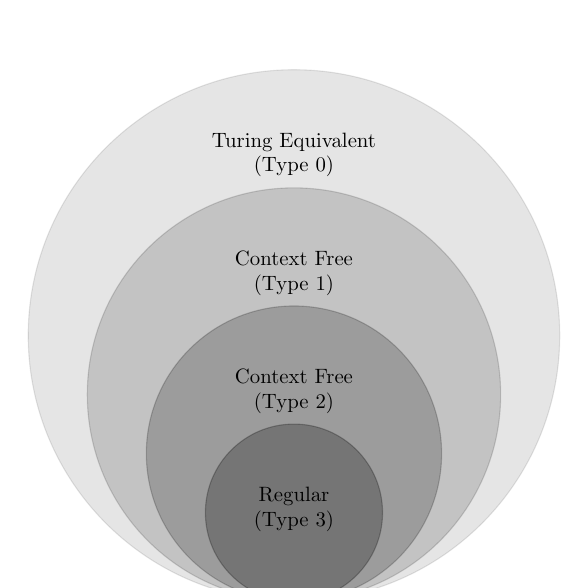
\begin{tikzpicture}[scale=0.75, every node/.style={scale=0.75},
	circ/.style={circle, draw, fill, minimum width=3cm},
	]
	
	\node[circ, opacity=0.25, label={[label distance=-1.95cm, align=center]90:Regular \\ (Type 3)}] (Reg) {};
	\node[circ, opacity=0.2, minimum width=5cm, above=0cm of Reg.south, label={[label distance=-1.95cm, align=center]90:Context Free \\ (Type 2)}] (CFG) {};
	\node[circ, opacity=0.15, minimum width=7cm, above=0cm of Reg.south, label={[label distance=-1.95cm, align=center]90:Context Free \\ (Type 1)}]  (CSG) {};
	\node[circ, opacity=0.1, minimum width=9cm, above=0cm of Reg.south, label={[label distance=-1.95cm, align=center]90:Turing Equivalent \\ (Type 0)}] (CSG) {};
	\end{tikzpicture}
	\caption[Chomsky Hierarchy]{A visual representation of the Chomsky Hierarchy.}
\label{fig:ChomskyHierarchy}
\end{figure}

The four types of formal grammars can be defined by the form their rules can take. An overview over these rules as per \cite{JurafskyMartin2009} can be found in Table \ref{tab:GrammarRules}, where $A$ is a single non-terminal, $\alpha$, $\beta$, $\gamma$ are strings of terminal and non-terminal symbols, and $x$ is a string of terminal symbols. $\alpha$, $\beta$ and $\gamma$ may be empty unless specifically disallowed. The table is supplemented with a column describing the corresponding automaton capable of accepting or recognizing the grammar.

\begin{table}[b]
	\begin{tabularx}{\textwidth}{@{}l*{10}{C}c@{}}
	\toprule 
	\textit{Type} & \textit{Name} & \textit{Rule Skeleton} & \textit{Automaton}\\ 
	\toprule	
	0 & Turing Equivalent & $\alpha \rightarrow \beta$, s.t. $\alpha \neq \epsilon$ & Turing Machine (recognized) \\
	1 & Context Sensitive & $\alpha A \beta \rightarrow \alpha \gamma \beta$, s.t. $\gamma \neq \epsilon$ &  Linear Bound Automata (accepted) \\
	2 & Context Free & $A \rightarrow \gamma$ & Push Down Automata (accepted) \\
	3 & Regular & $A \rightarrow xB$ or $A \rightarrow x$ & Finite-State Automata (accepted) \\
	\bottomrule	
	\end{tabularx}
	\caption[Formal grammar properties.]{Overview of formal grammar properties according to \cite{JurafskyMartin2009}, augmented with corresponding automata.}
	\label{tab:GrammarRules}
\end{table}

\subsection{Formal Grammars and Natural Language}
The correspondence of formal grammars to automata (i.e. Kleene's Theorem for regular languages and finite automata) and Computational Complexity Theory lends itself to consider natural languages under the same lense. While formal grammars constitute powerful tools with which phenomena in natural language can be modelled, assessing the precise complexity of Natural Language is the subject of ongoing investigation (\cite{Fitch2012}, \cite{Petersson2012}, \cite{Newmeyer2014}).
Arguments answering that question usually seek to establish lower bounds: If there is a phenomenon in a natural language that cannot be described with a given type of grammar, natural language must be - however slightly - more complex than that type allows. Such arguments increase in credibility the more frequently they can be replicated for phenomena in multiple languages. The arguments establishing natural languages as supra-context-free (i.e. more complex than CFGs) as well as contrary evidence from empiric research shall be presented here.

\subsubsection{Natural Language as supra-regular}\label{supraReg}
English, as well as several other languages (\cite{Hagege1976}) allow for center embedding, the embedding of a phrase into another phrase of the same type.
\begin{exe}
	\ex The man eats.
	\ex The man the boss fired eats.
	\ex The man the boss the investor distrusted fired eats.
	\ex The man the boss the investor the police investigated distrusted fired eats.
\end{exe}
Let the set $E$ contain all grammatical sentences of English, and let the noun phrases and transitive verbs constitute following sets:
\begin{align*}
A &= \lbrace \text{the boss}, \, \text{the investors}, \, \text{the police}, \dots \rbrace \\
B &= \lbrace \text{fired}, \, \text{distrusted}, \, \text{investigated}, \dots \rbrace
\end{align*}
Then the following two sets can be defined.
\begin{align*}
E' &= \lbrace \text{the man } a^{n}b^{n} \text{ eats} \: \vert \: n \geq 0 \rbrace \\
R &= \lbrace \text{the man } a^{*}b^{*} \text{ eats} \rbrace
\end{align*}
$a^{n}$ and $b^{n}$ are finite sequences of size $n$ of elements of sets $A$ and $B$, respectively. $E'$ describes a subset of $E$, namely $E \cap R$. Since regular languages are closed under intersection and $E'$ is not regular, $E$ is not regular.\footnote{The proofs for regular languages being closed under intersection and $E'$ not being regular can be found in \cite{Hopcroft2006} and \cite{Sipser2013}.}

While this proof is correct under the framework of Formal Language Theory, the validity of claiming that it shows natural language to be supra-regular is debatable. Research in psycholinguistics shows that native speakers have faced severe problems processing center embeddings of depth two or higher, yielding long processing times, an incomplete understanding of the presented sentence or leading the participants to judge the sentence as ungrammatical (\cite{Hamilton1971}, \cite{Frank2016}). Furthermore, the corpus-driven analysis by \cite{Karlsson2007} suggests an upper limit of center embedding depth three in the seven investigated languages.
% Keeping the following rant for posterity (or a future blog post)
%The proof concerns linguistic competence, whereas empirical studies provide an insight into linguistic performance. Usually, the distinction between competence and performance provide an adequate framework for both theoretical and empirical work, but when discussing the complexity of natural language neither side should be discarded. A linguistic competence framework cannot appropriately declare natural language as supra-regular if natural language is produced and processed according to regular rules. Conversely, for the purposes of computational linguistics, exclusively assessing linguistic performance by way of corpus analysis is insufficient, as a corpus of any size pales in comparison to the potential for infinitely many combinations that characterizes language. For the purposes of NLP, it is recommendable to err on the side of overestimating the complexity of natural language - so long as the resulting models are sufficiently efficient and accurate.

\subsubsection{Natural Language as supra-context-free}\label{supraCF}
Similarly to the proof given in Section \ref{supraReg}, an argument characterizing natural language as supra-context-free can be brought forth. It is based on embedded infinitival verb phrases found in Swiss German (\cite{Shieber1987}).
\begin{exe}
	\ex
	\gll Jan säit das mer em Hans es huus haend wele hälfe aastriiche. \\
	Jan said that we the Hans-DAT the house-ACC have wanted help paint \\
	\trans 'Jan said that we have wanted to help Hans paint the house.'
	\ex
	\gll Jan säit das mer d'chind em Hans es huus haend wele laa hälfe aastriiche. \\
	Jan said that we the children-ACC the Hans-DAT the house-ACC have wanted let help paint \\
	\trans 'Jan said that we have wanted to let the children help Hans paint the house.'
\end{exe}
Four finite sets can be constructed from these examples: accusative noun phrases ($A = \lbrace \text{d'chind}, \, \dots \rbrace$), dative noun phrases ($B = \lbrace \text{em Hans}, \, \dots \rbrace$), verbs taking accusative objects ($C = \lbrace \text{laa}, \, \dots \rbrace$) and verbs taking dative objects ($D = \lbrace \text{hälfe}, \, \dots \rbrace$). Let the set $S$ then be the set of all grammatical sentences of Swiss German. Again, the two following sets can be defined:
\begin{align*}
S' &= \lbrace \text{Jan säit das mer } a^{n}b^{m} \text{ es huus haend wele } c^{n}d^{m} \text{ aastriiche} \: \vert \: n, m \geq 0 \rbrace \\
R &= \lbrace \text{Jan säit das mer } a^{*}b^{*} \text{ es huus haend wele } c^{*}d^{*} \text{ aastriiche} \rbrace
\end{align*}
$S'$ is not context-free and results from $S \cap R$. Since context-free sets are closed under intersection with regular sets, $G$ cannot be context-free.\footnote{The respective proofs for $S'$ not being context-free and context-free sets being closed under intersection with regular sets can be found in \cite{Hopcroft2006} and \cite{Sipser2013}.}

Curiously enough, empirical research into the matter of processing similar cross-serial dependencies in Dutch suggests them to be generally easier to process than nested dependencies (i.e. the ones used to prove natural language to be supra-regular) (\cite{Bach1986}).

\subsection{Dyck Languages}\label{dyckLanguages}
Whether natural language is regular, context-free, supra-regular or supra-context-free is a distinction of only tangential relevance for this work. The first two cases are fully covered by CFGs, while the other two leave room for some natural language productions outside of the scope of CFGs. The characteristics of supra-context-free examples in natural language show a \textit{weak} non-context-freeness, making CFGs sufficient for covering the vast majority of natural language productions. With this assumption, an appropriate CFG for a model to learn must be found. The most important property of this grammar is that model performance on its language must allow for strong conclusions about the learnability of any other CFG. In doing so, one can make reasoned assumptions about potential model performance on natural language data. 

One such grammar is the Dyck Grammar, which can produce an array of Dyck Languages. Let $D_{n} = \lbrace N, \Sigma, R, S \rbrace$ with
\begin{align*}
	N &= \lbrace S \rbrace \\
	\Sigma &= \lbrace \epsilon, O_{1}, O_{2}, \dots, O_{n}, C_{1}, C_{2}, \dots, C_{n} \rbrace \\
	R &= \lbrace \\
		 & \qquad S \rightarrow \epsilon \\
		 & \qquad S \rightarrow SS \\
		 & \qquad S \rightarrow O_{n} \, S \, C_{n} \, \rbrace ,
\end{align*}
where $O_{n}$ represents an opening parenthesis, $C_{n}$ represents a closing parenthesis and $n$ denotes the number of distinct pairs of parentheses. $D_1$, then, denotes the Dyck Language with $\Sigma = \lbrace \epsilon, (, ) \rbrace$, $D_2$ the Dyck Language with $\Sigma = \lbrace \epsilon, (, [, ], ) \rbrace$, et cetera.

Within the family of Dyck Languages, $D_2$ is of particular interest. According to the Chomsky-Schützenberger Representation Theorem \citep{Chomsky1963}, for every context-free language $L$ there exists a positive integer $n$, a regular language $R$, and a homomorphism $h$ so that $L = h(D_{n} \cap R)$. Following the proof in \cite{Autebert1997}, a homomorphism $g_{n}$ can be constructed so that $D_{n} = g_{n}^{-1}(D_{2})$. It follows that every context-free language can be represented as $L = h(g_{n}^{-1}(D_{2}) \cap R)$. As such, every CFL could be represented via homomorphisms on $D_2$ and intersections with a regular language. Assuming natural languages to be context-free and bearing in mind that using a formal language is a choice of abstraction which allows for precise control over corpus composition, this makes $D_2$ the language of choice when comparing neural network performance.

\subsection{Neural Network Architectures}\label{neuralNetworkArchitectures}
\subsubsection{Simple RNN}\label{SRNN}
Recurrent Neural Networks (RNNs) (\cite{Elman1990}) are a neural network architecture particularly suited to processing sequential information by design: the RNN's output at a time step $t$ is fed back as its input at the following time step $t+1$. Not only does this enable RNNs to process sequences of arbitrary length, it also makes every output dependent on the previous computation as well as the current input. This property equips RNNs with a "memory" for previous inputs, allowing them to capture context dependencies a context-agnostic model cannot adequately learn.

Within the frame of this work, the specific case of the Simple RNN (SRNN) is considered. It is a three layer networks, consisting of an input layer, a hidden layer and an output layer. The hidden state $h_t$ at time step $t$ given the input vector $x_t$ and the output vector $y_t$ are calculated as per the following equations:
\begin{align}
	h_{t} &= f(\boldsymbol{W_{xh}} x_{t} + \boldsymbol{W_{hh}} h_{t-1}) \\
	y_{t} &= \boldsymbol{W_{hy}} h_{t}
\end{align}
The function $f$ constitutes a non-linear transformation, like $\tanh$ or ReLU. $\boldsymbol{W_{xh}}$, $\boldsymbol{W_{hh}}$, $\boldsymbol{W_{hy}}$ are matrices of the weights connecting the input layer to the hidden layer, the hidden layer to itself and the hidden layer to the output layer, respectively.

When training RNNs, it is beneficial to think of the network as unfolding into an architecture with one layer per time step. A visualisation is provided in Figure \ref{fig:unrolledRNN}. These conceptual layers share their parameters - if any weight changes at time step $t$, the weight also changes at $t+1, t+2, \dots, t+n$. Isolated changes are not possible. A popular training algorithm for RNNs is Backpropagation Through Time (BPTT) (\cite{Williams1998}), a gradient based algorithm designed for recurrent rather than feedforward networks. However, as \cite{Bengio1994} and \cite{Hochreiter1998} show, RNNs suffer from a fundamental flaw: the aptly named vanishing gradient problem, in which the training gradient diminishes to zero throughout the layers.

\begin{figure}[htb]
	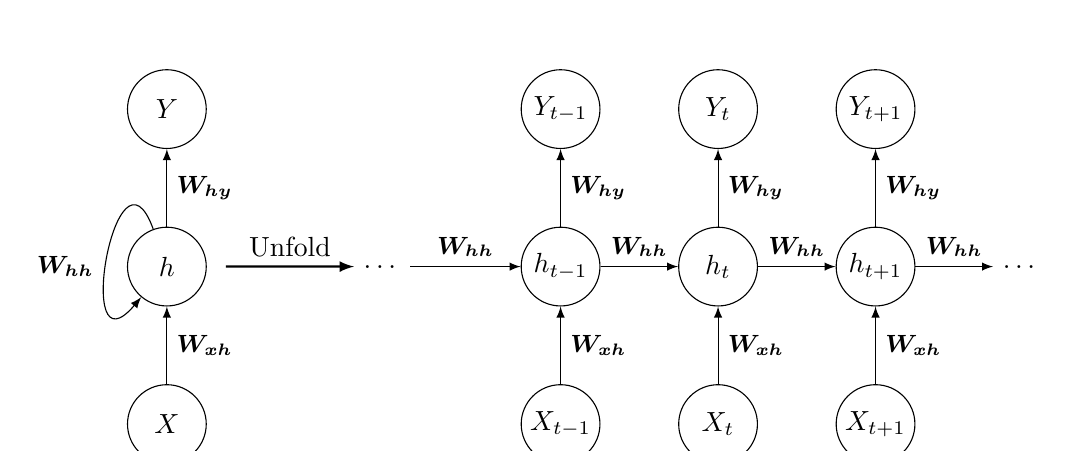
\begin{tikzpicture}[
    gt/.style={circle, draw, minimum width=1cm, minimum height=3mm, inner sep=1pt},
    ]
   	% Folded nodes
   	% Input
   	\node[gt] (X) {$X$};
   	% Hidden layer
	\node[gt, above=2cm of X.south] (h) {$h$};
	% Output layer
	\node[gt, above=2cm of h.south] (Y) {$Y$};
	
	% Unfolded nodes: t-1
   	% Input
   	\node[gt, right=5cm of X.west] (X_t-1) {$X_{t-1}$};
   	% Hidden layer
	\node[gt, right=5cm of h.west] (h_t-1) {$h_{t-1}$};
	% Output layer
	\node[gt, right=5cm of Y.west] (Y_t-1) {$Y_{t-1}$};
	% Unfolded nodes: t
   	% Input
   	\node[gt, right=2cm of X_t-1.west] (X_t) {$X_{t}$};
   	% Hidden layer
	\node[gt, right=2cm of h_t-1.west] (h_t) {$h_{t}$};
	% Output layer
	\node[gt, right=2cm of Y_t-1.west] (Y_t) {$Y_{t}$};
	% Unfolded nodes: t+1
   	% Input
   	\node[gt, right=2cm of X_t.west] (X_t+1) {$X_{t+1}$};
   	% Hidden layer
	\node[gt, right=2cm of h_t.west] (h_t+1) {$h_{t+1}$};
	% Output layer
	\node[gt, right=2cm of Y_t.west] (Y_t+1) {$Y_{t+1}$};

	% Implied prev/past nodes
	\node[left=1.4cm of h_t-1.west] (dots1) {\dots};
	\node[right=2cm of h_t+1.west] (dots2) {\dots};
	
	% Folded edges
	\draw[-latex] (X) -- (h) node[midway, right] {\small $\boldsymbol{W_{xh}}$};
	\draw[-latex] (h) -- (Y) node[midway, right] {\small $\boldsymbol{W_{hy}}$};
	\draw[-latex] (h) to [out=110, in=230 ,loop ,looseness=4.0] (h) node[left=0.3cm of h] {\small $\boldsymbol{W_{hh}}$};
	
	% Unfold arrow
	\draw[thick, -latex] (0.75, 2) -- (dots1) node[midway, above] {Unfold};
	
	% Unfolded edges t+1
	\draw[-latex] (X_t-1) -- (h_t-1) node[midway, right] {\small $\boldsymbol{W_{xh}}$};
	\draw[-latex] (h_t-1) -- (Y_t-1) node[midway, right] {\small $\boldsymbol{W_{hy}}$};
	
	% Unfolded edges t
	\draw[-latex] (X_t) -- (h_t) node[midway, right] {\small $\boldsymbol{W_{xh}}$};
	\draw[-latex] (h_t) -- (Y_t) node[midway, right] {\small $\boldsymbol{W_{hy}}$};
	
	% Unfolded edges t+1
	\draw[-latex] (X_t+1) -- (h_t+1) node[midway, right] {\small $\boldsymbol{W_{xh}}$};
	\draw[-latex] (h_t+1) -- (Y_t+1) node[midway, right] {\small $\boldsymbol{W_{hy}}$};
	
	% Unfolded edges h->h
	\draw[-latex] (dots1) -- (h_t-1) node[midway, above]  {\small $\boldsymbol{W_{hh}}$};
	\draw[-latex] (h_t-1) -- (h_t) node[midway, above]  {\small $\boldsymbol{W_{hh}}$};
	\draw[-latex] (h_t) -- (h_t+1) node[midway, above]  {\small $\boldsymbol{W_{hh}}$};
	\draw[-latex] (h_t+1) -- (dots2) node[midway, above]  {\small $\boldsymbol{W_{hh}}$};
	\end{tikzpicture}
 	\centering
 	\caption[Unfolded RNN]{An RNN, unfolded through time.}
	\label{fig:unrolledRNN}
\end{figure}

\subsubsection{LSTM}\label{LSTM}
Long-Short Term Memory networks (LSTM) were designed by \cite{Hochreiter1997} as an RNN architecture which preserves the RNN capabilities of processing sequential data of arbitrary length and capturing context dependencies, while circumventing the vanishing gradient problem.

LSTMs are based on self-connected linear units which are regulated by three gates consisting of a sigmoid layer $\sigma$ each: input (in), output (out) and forget (forget). At every time step, the concatenated vector of the previous hidden state $h_{t-1}$ and the current input $x_{t}$ are received by all three gates. The sigmoid layer transforms every value in the concatenated vector to a value in range $[0, \dots, 1]$ - a $0$ translates to forgetting the information, while a $1$ passes it through completely. Thus, the output of the gates determines what information is let through the input gate, passed through the output gate or forgotten by the self-connected linear unit.
\begin{align*}
\text{in}_{t} &= \sigma_{\text{in}} (\boldsymbol{W_{\text{in}}} \cdot [h_{t-1},x_{t}] + b_{\text{in}}) \\
\text{out}_{t} &= \sigma_{\text{out}} (\boldsymbol{W_{\text{out}}} \cdot [h_{t-1},x_{t}] + b_{\text{out}}) \\
\text{forget}_{t} &= \sigma_{\text{forget}} (\boldsymbol{W_{\text{forget}}} \cdot [h_{t-1},x_{t}] + b_{\text{forget}})
\end{align*}
Finally, the cell state $C_{t-1}$ is updated to $C_{t}$ and $h_{t}$ is set.
\begin{align*}
C_{t} &= \text{forget}_{t} \odot C_{t-1} + \text{in}_{t} \odot \tanh (\boldsymbol{W_{C}} \cdot [h_{t-1},x_{t}] + b_{\text{C}}) \\
h_{t} &= \text{out}_{t} \odot \tanh (C_{t})
\end{align*}
\begin{figure}[htb]
	\centering
	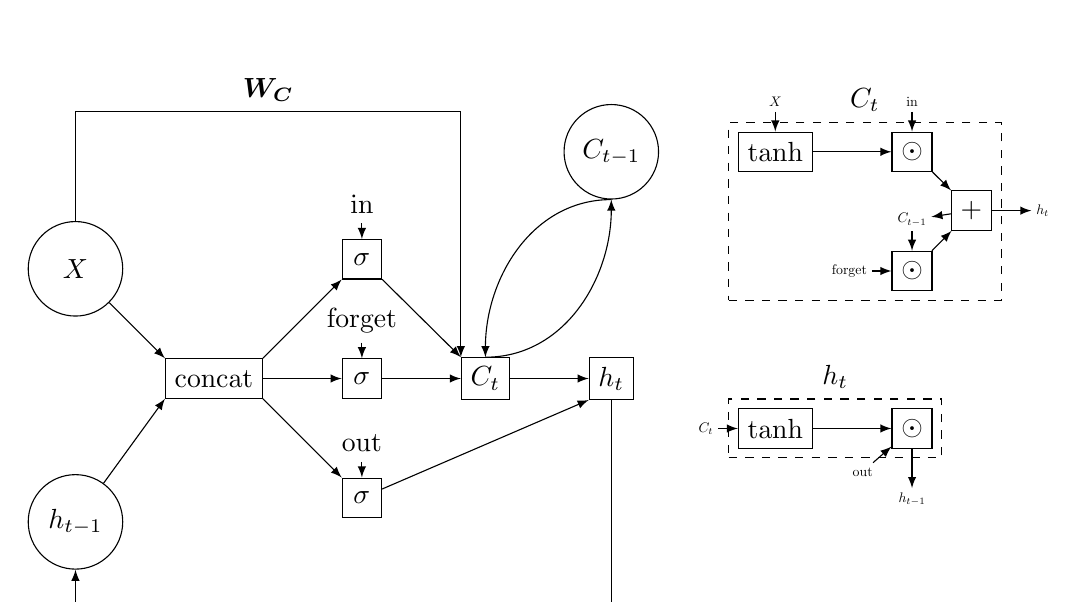
\begin{tikzpicture}[
    vec/.style={circle, draw, minimum width=1.2cm},
    op/.style={rectangle, draw, minimum width=0.5cm, minimum height=0.5cm},
    ]
    
   % Full LSTM
   \node[vec] (X) {$X$};
   \node[vec, below=2cm of X.south] (h_t-1) {$h_{t-1}$};
   
   \node[op, below right=1cm of X] (concat) {concat};
   
   \node[op, right=1cm of concat] (forget) {$\sigma$};
   \node[above=0.2cm of forget] (m_forget) {$\text{forget}$};
   \node[op, above=1cm of forget] (in) {$\sigma$};
   \node[above=0.2cm of in] (m_in) {$\text{in}$};
   \node[op, below=1cm of forget] (out) {$\sigma$};
   \node[above=0.2cm of out] (m_out) {$\text{out}$};
   
   \node[op, right=1cm of forget] (C_t) {$C_t$};
   \node[op, right=1cm of C_t] (h_t) {$h_{t}$};
   
   \node[vec, above=2cm of h_t] (C_t-1) {$C_{t-1}$};
   
   \draw[-latex] (X) -- (concat.north west);
   \draw[-latex] (h_t-1) -- (concat.south west);
   \draw[-latex] (concat.north east) -- (in);
   \draw[-latex] (concat) -- (forget);
   \draw[-latex] (concat.south east) -- (out);
   
   % Gate multiplicators.
   \draw[-latex] (m_in) -- (in);
   \draw[-latex] (m_forget) -- (forget);
   \draw[-latex] (m_out) -- (out);
   
   \draw[-latex] (in) -- (C_t.north west);
   \draw[-latex] (forget) -- (C_t);
   \draw[-latex] (out) -- (h_t.south west);
   
   \draw[-latex] (C_t) -- (h_t);
   
   \draw[-latex] (C_t-1.south) to [out=180,in=90] (C_t.north);
   \draw[-latex] (C_t.north) to [out=360,in=270] (C_t-1.south);
   
   \draw[-latex] (X) -- ++(0,2cm) -| (C_t.north west) node[pos=0.25, above] (W_c) {$\boldsymbol{W_{C}}$};
   
   \draw[-latex] (h_t) -- ++(0,-3cm) -| (h_t-1);
   
   % C_t close-up.
   \node[op, right=1cm of C_t-1] (tanh_c) {$\tanh$};
   \node[op, right=1cm of tanh_c] (mult_c1) {$\odot$};
   \node[op, below=1cm of mult_c1.south] (mult_c2) {$\odot$};
   \node[op, below right=0.33cm of mult_c1] (add_c) {$+$};
   \node[draw, dashed, fit=(tanh_c) (mult_c1) (mult_c2) (add_c), label={$C_{t}$}] {};
   \node[scale=0.5, above=0.25 of mult_c1] (in_c) {in};
   \node[scale=0.5, above=0.25 of tanh_c] (x_c) {$X$};
   \node[scale=0.5, left=0.25 of mult_c2] (forget_c) {forget};
   \node[scale=0.5, above=0.25 of mult_c2] (C_t-1_c) {$C_{t-1}$};
   \node[scale=0.5, right=0.5 of add_c] (h_t_c) {$h_{t}$};
      
   \draw[-latex] (x_c) -- (tanh_c.north);
   \draw[-latex] (in_c) -- (mult_c1);
   \draw[-latex] (forget_c) -- (mult_c2);
   \draw[-latex] (C_t-1_c) -- (mult_c2);
   
   \draw[-latex] (tanh_c) -- (mult_c1);
   \draw[-latex] (mult_c1) -- (add_c);
   \draw[-latex] (mult_c2) -- (add_c);
   
   \draw[-latex] (add_c) -- (h_t_c);
   \draw[-latex] (add_c) -- (C_t-1_c);
   
   % h_t close-up.
   \node[op, below=3cm of tanh_c] (tanh_h) {$\tanh$};
   \node[op, right=1cm of tanh_h] (mult_h) {$\odot$};
   \node[scale=0.5, left=0.25 of tanh_h] (C_h) {$C_{t}$};
   \node[scale=0.5, below left=0.25 of mult_h] (out_h) {out};
   \node[scale=0.5, below=0.5 of mult_h] (h_t-1_h) {$h_{t-1}$};
   \node[draw, dashed, fit=(tanh_h) (mult_h), label={$h_{t}$}] {};
   \draw[-latex] (C_h) -- (tanh_h);
   \draw[-latex] (out_h) -- (mult_h);
   
   \draw[-latex] (tanh_h) -- (mult_h);
   
   \draw[-latex] (mult_h) -- (h_t-1_h);
   
\end{tikzpicture}
	\caption[LSTM Memory Cell]{An LSTM memory cell.}
	\label{fig:memoryCellLSTM}
\end{figure}

\subsubsection{GRU}\label{GRU}
A less complex alternative to LSTMs, the Gated Recurrent Unit (GRU) was developed by \cite{Cho2014}. The information flow within the GRU is handled by just two gates: reset ($r$) and update ($z$). The update gate determines how much information from previous time steps is passed along for further time steps, while the reset gate enables the model to drop irrelevant information and only consider the current input rather than the previous hidden state, as described in the equations below, where $j$ is the $j$-th hidden unit, $\sigma$ is the squashing sigmoid function, $\boldsymbol{W}$ and $\boldsymbol{U}$ are learned gate-dependent weight matrices and $\phi$ is a non-linear function.
\begin{align*}
r_j &= \sigma \big( [\boldsymbol{W_{r}}x]_{j} + [\boldsymbol{U_{r}}h_{t-1}]_{j} \big) \\
z_j &= \sigma \big( [\boldsymbol{W_{z}}x]_{j} + [\boldsymbol{U_{z}}h_{t-1}]_{j} \big) \\
h_{j}^{t} &= z_{j}h_{j}^{t-1} + (1 - z_{j}) \tilde{h}_{j}^{t} \\
\tilde{h}_{j}^{t} &= \phi \big( [\boldsymbol{W}x]_{j} +[\boldsymbol{U}(r \odot h_{t-1})]_{j} \big)
\end{align*}

\begin{figure}[htb]
	\centering
	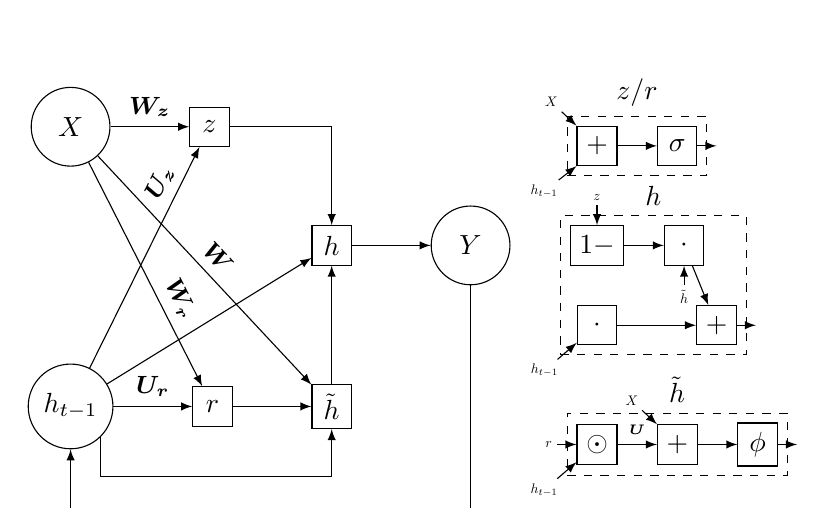
\begin{tikzpicture}[
    	vec/.style={circle, draw, minimum width=1cm},
    	op/.style={rectangle, draw, minimum width=0.5cm, minimum height=0.5cm},
    ]
    % Full GRU
    \node[vec] (X) {$X$};
    \node[vec, below=2.5cm of X] (h_t-1) {$h_{t-1}$};
    \node[op, right=1cm of X] (z) {$z$};
    \node[op, right=1cm of h_t-1] (r) {$r$};
    \node[op, right=1cm of r] (h_tilde) {$\tilde{h}$};
    \node[op, above=1.5cm of h_tilde] (h) {$h$};
    \node[vec, right=1cm of h] (Y) {$Y$};
    % Help nodes for clean edges
    \node[below right=1cm of h_t-1] (in_h_t-1) {};
    \coordinate[below=0.5cm of h_tilde] (in_h_tilde);
    
    
    % Edges z
    \draw[-latex] (X) -- (z) node[midway,above] {\small $\boldsymbol{W_{z}}$};
    \draw[-latex] (h_t-1) -- (z) node[sloped, pos=0.80, above] {\small $\boldsymbol{U_{z}}$};
    \draw[-latex] (z) -| (h);
    % Edges r
    \draw[-latex] (X) -- (r) node[sloped, pos=0.65, above] {\small $\boldsymbol{W_{r}}$};
    \draw[-latex] (h_t-1) -- (r) node[midway, above] {\small $\boldsymbol{U_{r}}$};
    \draw[-latex] (r) -- (h_tilde);
    \draw[-latex] (h_tilde) -- (h);
    \draw[-latex] (h_t-1.south east) -- ++(0,-0.5cm) -| (h_tilde.south);
    % Edges h_tilde
    \draw[-latex] (X) -- (h_tilde) node[sloped, midway, above] {\small $\boldsymbol{W}$};
    % Edges h
    \draw[-latex] (h_t-1) -- (h);
    \draw[-latex] (h) -- (Y);
    % Loop Output back to h_t-1
    \draw[-latex] (Y) -- ++(0,-3.5cm) -| (h_t-1.south);
    
    % Operator closeups
    %h closeup
    \node[op, right=0.75cm of Y] (1-) {$1-$};
    \node[op, right=0.5cm of 1-] (h_mult2) {$\cdot$};
    \node[op, below=0.5cm of 1-] (h_mult) {$\cdot$};
    \node[op, right=1cm of h_mult] (+h) {$+$};
    \node[scale=0.5, above=0.25cm of 1-] (z_h) {$z$};
    \node[scale=0.5, below=0.25cm of h_mult2] (h_tilde_h) {$\tilde{h}$};
    \node[scale=0.5, below left=0.25cm of h_mult] (h_t-1_h) {$h_{t-1}$};
    \node[draw, dashed, fit=(1-) (h_mult) (h_mult2) (+h), label={$h$}] {};
    \draw[-latex] (z_h) -- (1-);
    \draw[-latex] (1-) -- (h_mult2);
    \draw[-latex] (h_tilde_h) -- (h_mult2);
    \draw[-latex] (h_t-1_h) -- (h_mult);
    \draw[-latex] (h_mult) -- (+h);
    \draw[-latex] (h_mult2) -- (+h);
    \draw[-latex] (+h) -- ++(0.5cm,0);
    
    %h_tilde closeup
    \node[op, below=1cm of h_mult] (h_tilde_mult) {$\odot$};
    \node[op, right=0.5cm of h_tilde_mult] (+h_tilde) {$+$};
    \node[op, right=0.5cm of +h_tilde] (lin_h_tilde) {$\phi$};
    \node[scale=0.5, above left=0.25cm of +h_tilde] (x_h_tilde) {$X$};
    \node[scale=0.5, left=0.25cm of h_tilde_mult] (r_h_tilde) {$r$};
    \node[scale=0.5, below left=0.25cm of h_tilde_mult] (h_t-1_h_tilde) {$h_{t-1}$};
    \node[draw, dashed, fit=(h_tilde_mult) (+h_tilde) (lin_h_tilde), label={$\tilde{h}$}] {};
    \draw[-latex] (r_h_tilde) -- (h_tilde_mult);
    \draw[-latex] (h_t-1_h_tilde) -- (h_tilde_mult);
    \draw[-latex] (x_h_tilde) -- (+h_tilde.north west);
    \draw[-latex] (h_tilde_mult) -- (+h_tilde) node[midway, above] {\tiny $\boldsymbol{U}$};
    \draw[-latex] (+h_tilde) -- (lin_h_tilde);
    \draw[-latex] (lin_h_tilde) -- ++(0.5cm,0);
    
    % z
    \node[op, above=0.75cm of 1-] (+z) {$+$};
    \node[op, right=0.5cm of +z] (sigz) {$\sigma$};
    \node[scale=0.5, above left=0.25cm of +z] (x_z) {$X$};
    \node[scale=0.5, below left=0.25cm of +z] (h_t-1_z) {$h_{t-1}$};
    \node[draw, dashed, fit=(+z) (sigz), label={$z$/$r$}] {};
    \draw[-latex] (x_z) -- (+z.north west);
    \draw[-latex] (h_t-1_z) -- (+z.south west);
    \draw[-latex] (+z) -- (sigz);
    \draw[-latex] (sigz) -- ++(0.5cm,0);
\end{tikzpicture}
 \caption[Illustration of a GRU]{Illustration of a GRU.}
\label{fig:GRU}
\end{figure}

\subsection{Related Works}\label{relatedWorks}
Currently, NLP models are trained and tested on vast datasets, such as the CoNLL Shared Tasks. By evaluating a variety of different models and approaches on the same data, it is possible to easily assess which one poses the current state-of-the-art for any given NLP task.

The earliest research on neural network architectures was done before such datasets were widely available and easy to process (\cite{Cleeremans1989}, \cite{Elman1990}, \cite{Zeng1994}, \cite{Hochreiter1997}, \cite{Rodriguez1998}, \cite{GersSchmidhuber2001}). During that time, novel architectures and algorithms were mostly scored on formal language datasets, with the test set containing longer words than the training set to assess learning success. However, evaluating on formal languages comes with its own advantages and challenges.

Primarily, it is undeniably cheaper than scoring on a natural language dataset. By deriving words from the grammar, datasets of arbitrary length with arbitrary properties can be generated. However, performance on a formal grammar dataset should always be understood as a simplified benchmark. As mentioned in Sections \ref{supraReg} and \ref{supraCF}, the formal complexity of natural language is debatable, limiting the significance of formal benchmark performance for NLP tasks. Nevertheless, formal language datasets are still used to evaluate the performance of novel architectures to this day, as done by \cite{Joulin2015}, \cite{Bernardy2018}, \cite{Deleu2016}, \cite{Li2018} and \cite{Yu2019}.

In addition to the exploration of new architectures, formal languages are also still used to investigate particular behaviours of well-established architectures, such as LSTMs (\cite{Sennhauser2018}), or to compare several established models on a specific set of tasks (\cite{Skachkova2018}, \cite{Suzgun2019}).
\begin{table}
	\begin{tabularx}{\textwidth}{@{}l*{10}{C}c@{}}
		\toprule 		
		\textit{Paper} & \textit{D$_n$} & \textit{Grammar Probability} & \textit{Training Corpus Size} \\ 
		\toprule
		\cite{Deleu2016} & 1 & equal & unclear \\ 
		\cite{Bernardy2018} & 1, 5 & equal & $102,400$ \\ 
		\cite{Li2018} & 1 & modified & $200$ - $20,000$ \\ 
		\cite{Skachkova2018} & 1-5 & modified & $131,072$ \\ 
		\cite{Sennhauser2018} & 2 & modified & $1,000,000$ \\ 
		\cite{Suzgun2019} & 1-2 & modified & $10,000$ \\ 
		\cite{Yu2019} & 2 & modified & $1,000,000$ \\ 
		\bottomrule
	\end{tabularx}
	\caption[Corpus sizes in current works]{Overview of corpus sizes in current works.}
	\label{tab:LiteratureCorpusOverview}
\end{table}
\begin{table}
	\begin{tabularx}{\textwidth}{@{}l*{10}{C}c@{}}
	\toprule 
	\textit{Paper} & \textit{Accuracy} & \textit{Perplexity} & \textit{Cell State} & \textit{AUC} & \textit{Error Rate} \\
	\toprule
	\cite{Deleu2016} & No & No & No & Yes & No \\
	\cite{Bernardy2018} & Yes & No & No & No & No \\
	\cite{Skachkova2018} & Yes & Yes & No & No & No \\
	\cite{Sennhauser2018} & No & No & Yes & No & Yes \\
	\cite{Suzgun2019} & Yes & No & Yes & No & No\\
	\cite{Yu2019} & No & Yes & No & No & Yes \\ 
	\bottomrule
	\end{tabularx} 
	\caption[Reported values for performance in previous works]{Overview of reported values for performance. Cell State Analysis does not refer to a unified method, it merely means the paper investigates cell states at all. AUC refers to the area under the curve for an increasing length of Dyck words the model was able to generalize.}
	\label{tab:LiteratureReportedMeasures}
\end{table}
\begin{table}
	\begin{tabularx}{\textwidth}{@{}l*{10}{C}c@{}}
	\toprule 
	\textit{Paper} & \textit{Architectures} \\
	\toprule 
	\cite{Deleu2016} & Neural Turing Machine, LSTM \\
	\cite{Bernardy2018} & GRU, LSTM, RUSS \\
	\cite{Skachkova2018} & SRNN, GRU, LSTM \\
	\cite{Sennhauser2018} & LSTM \\
	\cite{Suzgun2019} & SRNN, GRU, LSTM \\
	\cite{Yu2019} & seq2seq \\ 
	\bottomrule
	\end{tabularx}
	\caption[Overview of investigated models]{Overview of investigated models.}
	\label{tab:LiteratureInvestigatedModels}
\end{table} 

While all these papers use a formal language to evaluate models, several factors prevent them from forming a solid basis upon which to compare their respective results:
First, there is neither a benchmark train/dev/test set for Dyck languages (as is standard for most machine learning tasks) (Table \ref{tab:LiteratureCorpusOverview}), nor a set of measures that is reported consistently throughout the literature (Table \ref{tab:LiteratureReportedMeasures}). Additionally, only two papers compare the three well-established architectures (SRNN, GRU, LSTM) directly (Table \ref{tab:LiteratureInvestigatedModels}).
Finally, the employed training and test measures are not unified - in \cite{Bernardy2018}, for example, the models are trained to predict the next letter in words of variable length at any given time step, while in \cite{Suzgun2019}, they predict the final letter of a word. Further model details, such as the inclusion of an Embedding and/or a Dropout layer or the number of hidden units also vary.

In conclusion, despite formal languages having been used to assess neural network model performance for decades, there is little to no comparative studies of SRNN, LSTM and GRU models performing on $D_{2}$. Any research comparing new architectures to any of these models does so with both varying training and testing methods, as well as with vastly differing corpora and as such cannot be directly compared with each other. This allows for no conclusive statement on the relative performance of these popular RNN architectures based on the current literature.
\section{Experiment Setup}\label{ch:experimentSetup}
\subsection{Evaluation}\label{evaluation}
Generating the words for the two experiments follows the procedure described by \cite{Bernardy2018} and will be explained in depth in the coming sections. Whereas the research put forth in his paper scrutinized the generative abilities of RNNs, I am investigating the models performing a classification task. As such, my training, test, validation and experiment data all consist of the same $1{:}1$ ratio of correct-to-incorrect words. Within the incorrect words, a distinction between superfluous opening or closing brackets is made, also at a ratio of $1{:}1$.

As such, a random guessing strategy would yield a baseline accuracy of $50\%$. A model is considered as having learned useful features from the training data if it scores above the baseline accuracy in the experiments. Furthermore, if the model has learned the underlying grammar of $D_{2}$, there should be no difference in accuracy for the two classes of incorrect words, as both of them do not belong to $D_{2}$, regardless of which bracket is replaced.

\subsection{Models}\label{models}
For the following experiments, the three RNN architectures described in Section \ref{neuralNetworkArchitectures} have been used. All models consist of an embedding layer, a single layer of size $n = \lbrace 2^{1}, 2^{2}, \dots, 2^{n} \rbrace$ and a dense layer of size $1$ with sigmoid activation. The activation value of the neuron in the dense layer acts as the output of the model: a value $\geq 0.5$ means the model classified the input as a correct word. The models were implemented in Tensorflow 2.0.\footnote{The source code can be found at \url {https://github.com/FyDob/BSc-Thesis}.}

All models were trained with the same parameters. The training data was received one word at a time, in batches of $512$. The loss was computed by binary cross-entropy, as is current standard for binary classification tasks. Furthermore, the Adam optimizer (\cite{Kingma2014}) was applied with a learning rate of $0.0001$. At the end of a training epoch, the models were evaluated for loss and accuracy on a validation set of $120{,}000$ words. The models were trained until their loss on the validation set did not lower by more than $0.0001$ for three consecutive epochs or for at most $100$ epochs. The models with the lowest validation loss were used for all experiments.

The models were trained on the same training data for both experiments. To answer the question of training data influence on model performance, three distinct sets of training data were used, yielding a total of $9 \times 3 \times 3 = 81$ (number of different hidden units $\times$ number of training corpora $\times$ number of different architectures) evaluated models.

\subsection{Corpus Construction}\label{corpusConstruction}
To investigate the influence of corpus composition on model performance, three corpora were created: a baseline corpus which is directly sampled from a subset of $D_{2}$, as well as two modifications of the baseline corpus: one impoverishing the training data from long-range dependencies (Low LRD) and one enriching the training data with more long-range dependencies (High LRD). The sampling and modification processes will be explained later in this section.

The experiments were explicitly designed to test the models' abilities to generalize based on the training data they encounter. As such, it is prudent to give consideration to which properties the training data might possess to facilitate or inhibit generalizability - properties such as length, maximum nesting depth (ND) and the maximum distance between a pair of opening and closing brackets (BD). ND is, in this case, defined as the highest number of unresolved open brackets preceding an open bracket in a given word (i.e. in the word \texttt{\{[\{\}]\}}, the square open bracket is at ND$=1$, and the curly open bracket is at ND$=2$, making the maximum ND of the word $2$). Maximum BD, then, is the highest number of characters between a pair of brackets in a word. In the previous example word, the maximum BD would be $4$. These measures are reported in Table \ref{tab:Corpora} in terms of averages and variance.

\begin{table}
	\begin{tabularx}{\textwidth}{@{}l*{10}{C}c@{}}
		\toprule 		
		\textit{Corpus} & \textit{Word Length} & \textit{maxND} & \textit{maxBD} \\ 
		\toprule 
		Baseline & $18.37$ ($6.36$) & $4.31$ ($1.22$) & $13.00$ ($16.02$) \\
		High LRD & $18.67$ ($4.75$) & $5.12$ ($1.04$) & $16.67$ ($4.75$) \\
		Low LRD & $17.54$ ($8.04$) & $3.92$ ($0.98$) & $10.58$ ($9.02$) \\
		\bottomrule
	\end{tabularx}
	\caption[Training corpora properties]{Properties of the three corpora the models were trained on, reported in averages (variance in brackets).}
	\label{tab:Corpora}
\end{table}

Furthermore, the training corpora were chosen to be a small slice of a comparatively large subset of $D_{2}$. To facilitate generalization, the training corpora consist of words of varying length. As discussed in Section \ref{relatedWorks}, previous works largely utilized similarly small language subsets and achieved encouraging results. For a discussion of Experiment $1$ and $2$ on a training corpus consisting of a majority of the target language, see \cite{Bernardy2018}.

In determining an eligible maximum length, a known fact about the size of $D_{n}$ subsets was utilized: a Dyck language $D_{n}$ contains $n^mC_{m}$ words of length $2m$, where $C_{m}$ is the $m$-th Catalan number (\cite{Skachkova2018}). It follows that a maximum length limit of $2m$ produces a set of size $\sum_{i=2}^{2m}n^{i}C_{i}$. For example, a maximum length of 20 in $D_{2}$ ($D_{2}^{\leq 20}$) yields $20{,}119{,}506$ words, which is a sufficiently large subset to sample from. The words were generated following the probabilistic grammar set forth by \cite{Sennhauser2018}.
\begin{align*}
	S &\rightarrow Z \; S \; \vert \; Z \\
	Z &\rightarrow B \; \vert \; T \\
	B &\rightarrow [ \; S \; ] \; \vert \; \lbrace \; S \; \rbrace \\
	T &\rightarrow [ \; ] \; \vert \; \lbrace \; \rbrace
\end{align*}
The production $Z \rightarrow B$ branches, whereas $S \rightarrow Z \; S$ concatenates two smaller Dyck words. This representation provides a good intuition for understanding the merit of Experiment 1. The probabilities with which the rules were applied are calculated as follows, with alternative rules of course being applied with the complementary probability:
\begin{align*}
	P_{\text{branch}} &= r_{\text{branch}} \cdot s(l) \quad \text{with } r_{\text{branch}} \sim U(0.7,1.0) \\
	P_{\text{concat}} &= r_{\text{concat}} \cdot s(l) \quad \text{with } r_{\text{concat}} \sim U(0.7,1.0) \\
	s(l) &= \min(1, -3 \cdot \frac{l}{n} + 3)
\end{align*}
with $l$ being the number of already generated non-terminal characters and $n$ the maximally desired length of the word. $r_{\text{branch}}$, $r_{\text{concat}}$ and $l$ were sampled at every step of word generation.

Following this process, $500{,}000$ words in $D_{2}^{\leq 20}$ were generated. These words served as the basis for creating the three corpora. To create the Low LRD corpus, all words with a maximum bracket distance higher than $10$ were modified\footnote{This cut-off point was chosen as it significantly reduces the average maximum bracket distance without creating too many duplicates.} by first identifying the bracket pair with the highest bracket distance, then simply moving the opening bracket from its original position to the position right before the closing bracket. (i.e. \texttt{\{[\{\}]\}} becomes \texttt{[\{\}]\{\}}). This has the largest impact on bracket distance throughout the corpus, while ensuring grammaticality of the resulting word. The resulting set of long-range impoverished words was merged with all unmodified words, deleting all duplicates.

The High LRD corpus was created in a similar way: First, all words with a bracket distance lower than $19$ were identified.\footnote{The same considerations as for the Low LRD corpus cut-off apply.} Then, the first pair of neighbouring closing brackets is found and deleted. The remaining word is wrapped in a randomly chosen pair of brackets, creating the longest possible bracket distance between the two (i.e. \texttt{\{[\{\}]\}} becomes \texttt{\{\{[]\}\}}). The resulting set was merged with the unmodified words the same way as the Low LRD set.

Finally, the corpora were filled with $500{,}000$ non-words obtained by corrupting the correct words in $D_{2}^{\leq 20}$. For one half of the words, a random opening bracket was replaced with a random closing bracket, while a random closing bracket was replaced with a random opening bracket for the other half.

In total, all corpora consist of $1{,}000{,}000$ samples, of which $50\%$ are incorrect.

\subsection{Experiment 1: Long-Range Dependency}\label{LRD}
For this experiment, the test set consisted of $1{,}000{,}000$ samples of length $1+18+18+1=38$, half of which were correct Dyck words. They were created by picking two random Dyck words $w_{1}, w_{2} \in D_{2}^{=18}$ from the base corpus, concatenating them and wrapping the result in a randomly selected pair of matching brackets as follows:
\[
	w_{\text{LRD}} = O_{n}w_{1}w_{2}C_{n}
\]
To generate incorrect samples, the generated correct LRD words were corrupted in the same way as for the training corpora, yielding $250{,}000$ incorrect LRD words with a superfluous opening or closing bracket each.

While $w_{1}$ and $w_{2}$ might have been seen in training (for models trained on the base corpus), the resulting word most certainly has not been observed. Neither could the model possibly have encountered a long-range dependency spanning $36$ characters between the opening and closing bracket. As such, a high classification accuracy serves as a strong indication of the model having learned to generalize to longer, non-concatenated Dyck words.\footnote{While the infixed sub-words are indeed concatenated, $w_{\text{LRD}}$ cannot be created by concatenating two shorter words due to being wrapped by a matching bracket pair.} I report model performance on Experiment 1 in terms of accuracy, precision, recall and F1 score.

\subsection{Experiment 2: Deeper Nesting}\label{DN}
To investigate how well a model performs on predicting brackets on a nesting level deeper than anything included in training, another test set was constructed. Since Experiment 1 already investigates Long-Range Dependency (LRD), this corpus was designed so its results are confounded as little as possible by LRD performance.

For this task, the test set consisted of  $1{,}000{,}000$ samples of length $30$, half of which were correct Dyck words. First, $500,000$  correct words were chosen at random from the base corpus. Then, they were wrapped by a prefix of five randomly chosen opening brackets and a suffix of the corresponding closing brackets as follows:
\[
	w_{\text{DN}} = O_{n}O_{n}O_{n}O_{n}O_{n}wC_{n}C_{n}C_{n}C_{n}C_{n}
\]
Generation of incorrect samples was done in accordance to Experiment 1 and corpus creation.

This process still has the model extrapolate beyond the length of the training words, while increasing all present nesting depths by $5$. This is analogous to center embedding in natural language - processing increasing nesting levels is more complicated than processing a flat structure. A high classification accuracy in Experiment 2 indicates a capability to generalize to repeated application of grammar rules beyond what was seen in the training set. As such, it implies an understanding of the $D_{2}$ grammar. I report model performance on Experiment 2 in terms of accuracy, precision, recall and F1 score.
\section{Results}\label{ch:results}
During training, almost all $81$ trained models achieved a validation accuracy significantly above random guessing, except for the SRNN-2 models trained on the base and low LRD corpus, which scored $75.0\%$ and $50.4\%$ respectively. I have included them in the experiments regardless of their low validation accuracy, since it was unclear whether validation accuracy was a strong predictor for a network's performance on the experiment data. I present my results with regard to three focus points: First, the overall performance of different architectures with respect to which corpus they were trained on, then the individual model performances on each of the two experiments, and finally a closer look at classifications made by outlier networks - networks which drastically over- or underperformed in either of the experiments - with regards to word features.

\subsection{Architecture/Training Data}
\begin{table}
\begin{tabularx}{\textwidth}{@{}l*{10}{C}c@{}}
 \toprule
  & \textit{Accuracy} &  \textit{Precision} &  \textit{Recall} &  \textit{F1 Score} &  \textit{Val Acc} \\
 \midrule
 SRNN & \multicolumn{5}{c}{Base} \\
 \midrule
	Mean & \textit{0.476} & \textit{0.278} & \textit{0.181} & \textit{0.193} & 0.972 \\
	Variance & 0.064 & 0.235 & 0.257 & 0.220 & 0.081 \\
 \midrule
 SRNN & \multicolumn{5}{c}{Low LRD} \\
 \midrule
	Mean & \textbf{0.514} & \textbf{0.443} & \textbf{0.288} & \textbf{0.316} & \textit{0.932} \\
	Variance & 0.055 & 0.176 & 0.259 & 0.213 & 0.158 \\
 \midrule
 SRNN & \multicolumn{5}{c}{High LRD} \\
 \midrule
	Mean & 0.511 & 0.415 & 0.153 & 0.200 & \textbf{0.981} \\
	Variance & 0.043 & 0.211 & 0.171 & 0.187 & 0.054 \\
 \midrule
 SRNN & \multicolumn{5}{c}{Complete} \\
 \midrule
	Mean & \textit{0.500} & 0.379 & \textbf{0.208} & \textbf{0.236} & \textit{0.962} \\
	Variance & 0.056 & 0.217 & 0.236 & 0.211 & 0.107 \\
 \midrule
 \midrule
 LSTM & \multicolumn{5}{c}{Base} \\
 \midrule
 Mean & \textbf{0.543} & \textit{0.219} & 0.148 & 0.154 & 0.999 \\
Variance & 0.173 & 0.365 & 0.335 & 0.341 & 0.003 \\
 \midrule
 LSTM & \multicolumn{5}{c}{Low LRD} \\
 \midrule
 Mean & 0.529 & \textbf{0.391} & \textbf{0.176} & \textbf{0.195} & 0.999 \\
Variance & 0.158 & 0.295 & 0.311 & 0.302 & 0.002 \\
 \midrule
 LSTM & \multicolumn{5}{c}{High LRD} \\
 \midrule
 Mean & \textit{0.472} & 0.258 & \textit{0.036} & \textit{0.059} & \textbf{1.000} \\
Variance & 0.075 & 0.278 & 0.057 & 0.090 & 0.000 \\
 \midrule
 LSTM & \multicolumn{5}{c}{Complete} \\
 \midrule
Mean & 0.515 & \textit{0.289} & \textit{0.120} & \textit{0.136} & \textbf{0.999} \\
Variance & 0.143 & 0.318 & 0.268 & 0.269 & 0.002 \\
 \midrule
 \midrule
 GRU & \multicolumn{5}{c}{Base} \\
 \midrule
 Mean & 0.531 & \textit{0.371} & 0.147 & 0.185 & 0.999 \\
Variance & 0.097 & 0.297 & 0.226 & 0.247 & 0.001 \\
 \midrule
 GRU & \multicolumn{5}{c}{Low LRD} \\
 \midrule
 Mean & \textbf{0.554} & \textbf{0.507} & \textbf{0.206} & \textbf{0.243} & 0.999 \\
Variance & 0.133 & 0.198 & 0.302 & 0.285 & 0.001 \\
 \midrule
 GRU & \multicolumn{5}{c}{High LRD} \\
 \midrule
 Mean & \textit{0.514} & 0.439 & \textit{0.126} & \textit{0.170} & \textit{0.972} \\
Variance & 0.082 & 0.223 & 0.198 & 0.193 & 0.055 \\
 \midrule
 GRU & \multicolumn{5}{c}{Complete} \\
 \midrule
Mean & \textbf{0.533} & \textbf{0.439} & 0.160 & 0.200 & 0.990 \\
Variance & 0.106 & 0.245 & 0.244 & 0.242 & 0.034 \\
\bottomrule
\end{tabularx}
\caption[Performance measures for all networks]{Performance measures of all architectures across both experiments depending on which corpus they were trained on, as well as the compounded measures for all networks regardless of training data.}
\label{tab:perf_all}
\end{table}
As can be seen in Table \ref{tab:perf_all}, none of the architectures consistently achieved an accuracy far above the random guessing baseline of $50.0\%$. However, there was still a notable difference in performance between architectures: on average, the GRU networks scored the highest on accuracy and precision, while the SRNN networks achieved the best recall and F1 score. With $51.5\%$, LSTMs scored an average accuracy right between SRNNs ($50.0\%$) and GRUs ($53.3\%$), but they underperformed in all other experiment measures.

Futhermore, the choice of training data had a notable effect on overall model performance: SRNNs and GRUs received a boost in performance in all measures when comparing the Base to the Low LRD models, elevating SRNNs from an accuracy below random guessing to $51.4\%$. While LSTMs lost $1.4\%$ in terms of accuracy, all other performance measures improved significantly for the Low LRD models. Training on the High LRD corpus aided SRNNs in terms of accuracy, precision and F1 score, but worsened accuracy, recall and F1 score for LSTMs and GRUs.

\subsection{Experiment 1: Long-Range Dependency}\label{resultsLRD}
Bla bla bla

\begin{table}
\begin{tabularx}{\textwidth}{@{}l*{10}{C}c@{}}
\toprule
  \textit{Network} &  \textit{Accuracy} &  \textit{Precision} &  \textit{Recall} &  \textit{F1 Score} &  \textit{Val Acc} \\
\midrule
    GRU-2 &     0.890 &      \textbf{0.982} &   0.794 &     0.878 &    0.995 \\
    GRU-4 &     0.487 &      0.413 &   0.060 &     0.105 &    1.000 \\
    GRU-8 &     0.488 &      0.331 &   0.023 &     0.043 &    1.000 \\
   GRU-16 &     0.550 &      0.713 &   0.168 &     0.272 &    1.000 \\
   GRU-32 &     0.434 &      0.267 &   0.075 &     0.118 &    1.000 \\
   GRU-64 &     0.510 &      0.537 &   0.149 &     0.234 &    1.000 \\
  GRU-128 &     0.553 &      0.611 &   0.293 &     0.396 &    0.999 \\
  GRU-256 &     0.497 &      0.364 &   0.009 &     0.018 &    1.000 \\
  GRU-512 &     0.500 &      0.487 &   0.007 &     0.015 &    1.000 \\
   LSTM-2 &     0.500 &      0.000 &   0.000 &     0.000 &    0.999 \\
   LSTM-4 &     0.451 &      0.000 &   0.000 &     0.000 &    1.000 \\
   LSTM-8 &     \textbf{0.910} &      0.959 &   \textbf{0.857} &     \textbf{0.905} &    \textbf{1.000} \\
  LSTM-16 &     0.343 &      0.001 &   0.000 &     0.000 &    1.000 \\
  LSTM-32 &     0.500 &      0.000 &   0.000 &     0.000 &    1.000 \\
  LSTM-64 &     0.505 &      0.596 &   0.030 &     0.057 &    1.000 \\
 LSTM-128 &     0.347 &      0.001 &   0.000 &     0.000 &    1.000 \\
 LSTM-256 &     0.455 &      0.128 &   0.016 &     0.028 &    1.000 \\
 LSTM-512 &     0.499 &      0.468 &   0.009 &     0.017 &    0.991 \\
   SRNN-2 &     $0.465$ &      0.357 &   0.087 &     0.140 &    \textit{0.750} \\
   SRNN-4 &     $0.488$ &      0.334 &   0.023 &     0.043 &    1.000 \\
   SRNN-8 &     $0.461$ &      0.037 &   0.003 &     0.006 &    1.000 \\
  SRNN-16 &     $\textit{0.272}$ &      0.021 &   0.010 &     0.014 &    1.000 \\
  SRNN-32 &     0.498 &      0.492 &   0.141 &     0.219 &    1.000 \\
  SRNN-64 &     0.504 &      0.505 &   0.366 &     0.424 &    1.000 \\
 SRNN-128 &     0.484 &      0.040 &   0.001 &     0.003 &    1.000 \\
 SRNN-256 &     0.503 &      0.503 &   0.455 &     0.478 &    1.000 \\
 SRNN-512 &     0.484 &      0.017 &   0.001 &     0.001 &    1.000 \\
 \midrule
 \midrule
 \textbf{Mean} & 0.503 & 0.339 & 0.132 & 0.163 & 0.990 \\
 \textbf{Variance} & 0.130 & 0.294 & 0.233 & 0.253 & 0.048 \\
\bottomrule
\end{tabularx}
\caption[Base LRD trained network performance on experiment 1]{Performance measures for experiment 1 of all networks that were trained on the base LRD corpus.}
\label{tab:perf_LRDbase}
\end{table}
%\end%{tabularx}
%\caption[]{}
%\label{tab:perf}

\begin{tabular}{lrrrrr}
\toprule
  network &  accuracy &  precision &  recall &  f1\_score &  val\_acc \\
\midrule
    GRU-2 &     0.583 &      0.582 &   0.589 &     0.585 &    1.000 \\
    GRU-4 &     0.505 &      0.518 &   0.135 &     0.214 &    1.000 \\
    GRU-8 &     0.498 &      0.491 &   0.106 &     0.175 &    0.997 \\
   GRU-16 &     0.503 &      0.528 &   0.060 &     0.107 &    1.000 \\
   GRU-32 &     0.505 &      0.525 &   0.100 &     0.168 &    1.000 \\
   GRU-64 &     0.890 &      0.869 &   0.918 &     0.893 &    1.000 \\
  GRU-128 &     0.484 &      0.324 &   0.030 &     0.054 &    1.000 \\
  GRU-256 &     0.500 &      0.496 &   0.039 &     0.072 &    1.000 \\
  GRU-512 &     0.500 &      0.435 &   0.002 &     0.004 &    0.997 \\
   LSTM-2 &     0.500 &      0.500 &   0.475 &     0.487 &    0.996 \\
   LSTM-4 &     0.278 &      0.000 &   0.000 &     0.000 &    1.000 \\
   LSTM-8 &     0.500 &      0.000 &   0.000 &     0.000 &    1.000 \\
  LSTM-16 &     0.881 &      0.853 &   0.920 &     0.885 &    1.000 \\
  LSTM-32 &     0.491 &      0.092 &   0.002 &     0.004 &    1.000 \\
  LSTM-64 &     0.500 &      0.505 &   0.010 &     0.020 &    1.000 \\
 LSTM-128 &     0.496 &      0.374 &   0.011 &     0.021 &    0.998 \\
 LSTM-256 &     0.500 &      0.535 &   0.007 &     0.014 &    1.000 \\
 LSTM-512 &     0.507 &      0.566 &   0.058 &     0.106 &    1.000 \\
   SRNN-2 &     0.501 &      0.501 &   0.366 &     0.423 &    0.504 \\
   SRNN-4 &     0.708 &      0.646 &   0.922 &     0.760 &    0.930 \\
   SRNN-8 &     0.508 &      0.527 &   0.150 &     0.234 &    1.000 \\
  SRNN-16 &     0.500 &      0.000 &   0.000 &     0.000 &    1.000 \\
  SRNN-32 &     0.486 &      0.388 &   0.050 &     0.088 &    1.000 \\
  SRNN-64 &     0.487 &      0.375 &   0.040 &     0.072 &    1.000 \\
 SRNN-128 &     0.492 &      0.484 &   0.236 &     0.318 &    0.953 \\
 SRNN-256 &     0.501 &      0.501 &   0.412 &     0.452 &    1.000 \\
 SRNN-512 &     0.503 &      0.503 &   0.497 &     0.500 &    1.000 \\
\bottomrule
\end{tabular}


\begin{table}[t]
\begin{tabularx}{\textwidth}{@{}l*{10}{C}c@{}}
 \toprule
  \textit{Network} &  \textit{Accuracy} &  \textit{Precision} &  \textit{Recall} &  \textit{F1 Score} &  \textit{Val Acc} \\
 \midrule
    GRU-2 &     0.494 &      0.480 &   0.136 &     0.212 &    1.000 \\
    GRU-4 &     0.499 &      0.482 &   0.036 &     0.066 &    1.000 \\
    GRU-8 &     0.342 &      0.000 &   0.000 &     0.000 &    1.000 \\
   GRU-16 &     0.523 &      0.590 &   0.153 &     0.242 &    1.000 \\
   GRU-32 &     0.504 &      0.521 &   0.093 &     0.158 &    1.000 \\
   GRU-64 &     0.504 &      0.522 &   0.088 &     0.150 &    1.000 \\
  GRU-128 &     0.489 &      0.419 &   0.056 &     0.098 &    1.000 \\
  GRU-256 &     0.503 &      0.549 &   0.035 &     0.066 &    0.902 \\
  GRU-512 &     \textbf{0.800} &      \textbf{0.768} &   \textbf{0.861} &     \textbf{0.812} &    0.849 \\
   LSTM-2 &     0.483 &      0.390 &   0.060 &     0.104 &    1.000 \\
   LSTM-4 &     \textit{0.282} &      \textit{0.000} &   \textit{0.000} &     \textit{0.000} &    1.000 \\
   LSTM-8 &     0.379 &      0.000 &   0.000 &     0.000 &    1.000 \\
  LSTM-16 &     0.502 &      0.640 &   0.007 &     0.015 &    1.000 \\
  LSTM-32 &     0.498 &      0.475 &   0.038 &     0.070 &    1.000 \\
  LSTM-64 &     0.500 &      0.000 &   0.000 &     0.000 &    1.000 \\
 LSTM-128 &     0.492 &      0.365 &   0.022 &     0.041 &    1.000 \\
 LSTM-256 &     0.497 &      0.367 &   0.008 &     0.016 &    1.000 \\
 LSTM-512 &     0.500 &      0.000 &   0.000 &     0.000 &    0.999 \\
   SRNN-2 &     0.500 &      0.499 &   0.042 &     0.078 &    \textit{0.833} \\
   SRNN-4 &     0.502 &      0.523 &   0.046 &     0.085 &    0.996 \\
   SRNN-8 &     0.539 &      0.622 &   0.201 &     0.304 &    1.000 \\
  SRNN-16 &     0.500 &      0.000 &   0.000 &     0.000 &    0.999 \\
  SRNN-32 &     0.500 &      0.497 &   0.037 &     0.070 &    1.000 \\
  SRNN-64 &     0.503 &      0.504 &   0.360 &     0.420 &    1.000 \\
 SRNN-128 &     0.497 &      0.494 &   0.235 &     0.318 &    1.000 \\
 SRNN-256 &     0.496 &      0.495 &   0.340 &     0.403 &    1.000 \\
 SRNN-512 &     0.490 &      0.459 &   0.112 &     0.180 &    1.000 \\
 \midrule
 \midrule
 \textbf{Mean} & 0.493 & 0.395 & 0.110 & 0.145 & 0.984 \\
 \textbf{Variance} & 0.083 & 0.230 & 0.180 & 0.182 & 0.045 \\
 \bottomrule
\end{tabularx}
\caption[Experiment 1: High LRD network performance]{Performance measures for Experiment 1 of all networks that were trained on the High LRD corpus.}
\label{tab:perf_LRDhigh}
\end{table}

\subsection{Experiment 2: New Depths}\label{resultsND}

\begin{table}
\begin{tabularx}{\textwidth}{@{}l*{10}{C}c@{}}
\toprule
  \textit{Network} &  \textit{Accuracy} &  \textit{Precision} &  \textit{Recall} &  \textit{F1 Score} &  \textit{Val Acc} \\
 \midrule
    GRU-2 &     0.500 &      0.000 &   0.000 &     0.000 &    0.995 \\
    GRU-4 &     0.563 &      0.655 &   0.265 &     0.377 &    1.000 \\
    GRU-8 &     0.472 &      0.164 &   0.014 &     0.025 &    1.000 \\
   GRU-16 &     0.500 &      0.000 &   0.000 &     0.000 &    1.000 \\
   GRU-32 &     0.500 &      0.000 &   0.000 &     0.000 &    1.000 \\
   GRU-64 &     0.515 &      0.550 &   0.160 &     0.248 &    1.000 \\
  GRU-128 &     0.496 &      0.000 &   0.000 &     0.000 &    0.999 \\
  GRU-256 &     0.500 &      0.000 &   0.000 &     0.000 &    1.000 \\
  GRU-512 &     0.601 &      0.597 &   0.620 &     0.608 &    1.000 \\
   LSTM-2 &     0.500 &      0.000 &   0.000 &     0.000 &    0.999 \\
   LSTM-4 &     0.500 &      0.000 &   0.000 &     0.000 &    1.000 \\
   LSTM-8 &     0.500 &      0.000 &   0.000 &     0.000 &    1.000 \\
  LSTM-16 &     0.500 &      0.000 &   0.000 &     0.000 &    1.000 \\
  LSTM-32 &     0.778 &      0.792 &   0.755 &     0.773 &    1.000 \\
  LSTM-64 &     0.500 &      0.000 &   0.000 &     0.000 &    1.000 \\
 LSTM-128 &     \textbf{0.993} &      \textbf{0.991} &   \textbf{0.995} &     \textbf{0.993} &    \textbf{1.000} \\
 LSTM-256 &     0.500 &      0.000 &   0.000 &     0.000 &    1.000 \\
 LSTM-512 &     0.499 &      0.000 &   0.000 &     0.000 &    0.991 \\
   SRNN-2 &     0.580 &      0.548 &   0.917 &     0.686 &    \textit{0.750} \\
   SRNN-4 &     0.488 &      0.000 &   0.000 &     0.000 &    1.000 \\
   SRNN-8 &     0.500 &      0.000 &   0.000 &     0.000 &    1.000 \\
  SRNN-16 &     0.500 &      0.000 &   0.000 &     0.000 &    1.000 \\
  SRNN-32 &     0.515 &      0.564 &   0.136 &     0.220 &    1.000 \\
  SRNN-64 &     0.511 &      0.529 &   0.192 &     0.281 &    1.000 \\
 SRNN-128 &     0.441 &      0.409 &   0.266 &     0.322 &    1.000 \\
 SRNN-256 &     \textit{0.382} &      0.156 &   0.053 &     0.080 &    1.000 \\
 SRNN-512 &     0.497 &      0.497 &   0.615 &     0.550 &    1.000 \\
 \midrule
 \midrule
 \textbf{Mean} & 0.531 & 0.239 & 0.185 & 0.191 & 0.990 \\
 \textbf{Variance} & 0.113 & 0.311 & 0.308 & 0.290 & 0.048 \\
\bottomrule
\end{tabularx}
\caption[Base LRD trained network performance on experiment 2]{Performance measures for experiment 2 of all networks that were trained on the base LRD corpus.}
\label{tab:perf_NDbase}
\end{table}

\begin{table}[t]
\begin{tabularx}{\textwidth}{@{}l*{10}{C}c@{}}
\toprule
  \textit{Network} &  \textit{Accuracy} &  \textit{Precision} &  \textit{Recall} &  \textit{F1 Score} &  \textit{Val Acc} \\
\midrule
    GRU-2 &     0.494 &      0.488 &   0.222 &     0.306 &    1.000 \\
    GRU-4 &     0.561 &      0.651 &   0.262 &     0.374 &    1.000 \\
    GRU-8 &     0.499 &      0.492 &   0.056 &     0.101 &    0.997 \\
   GRU-16 &     0.497 &      0.465 &   0.039 &     0.072 &    1.000 \\
   GRU-32 &     0.500 &      0.000 &   0.000 &     0.000 &    1.000 \\
   GRU-64 &     0.935 &      0.910 &   0.966 &     0.937 &    1.000 \\
  GRU-128 &     0.516 &      0.560 &   0.144 &     0.229 &    1.000 \\
  GRU-256 &     0.499 &      0.486 &   0.043 &     0.078 &    1.000 \\
  GRU-512 &     0.497 &      0.305 &   0.004 &     0.008 &    0.997 \\
   LSTM-2 &     0.499 &      0.000 &   0.000 &     0.000 &    0.996 \\
   LSTM-4 &     0.480 &      0.328 &   0.037 &     0.067 &    1.000 \\
   LSTM-8 &     0.555 &      0.660 &   0.226 &     0.337 &    1.000 \\
  LSTM-16 &     0.566 &      0.662 &   0.270 &     0.384 &    1.000 \\
  LSTM-32 &     \textit{0.327} &      0.207 &   0.122 &     0.154 &    1.000 \\
  LSTM-64 &     0.491 &      0.301 &   0.014 &     0.026 &    1.000 \\
 LSTM-128 &     0.500 &      0.000 &   0.000 &     0.000 &    0.998 \\
 LSTM-256 &     0.502 &      0.538 &   0.027 &     0.051 &    1.000 \\
 LSTM-512 &     \textbf{0.953} &      \textbf{0.917} &   \textbf{0.996} &     \textbf{0.955} &    \textbf{1.000} \\
   SRNN-2 &     0.501 &      0.501 &   0.585 &     0.540 &    \textit{0.504} \\
   SRNN-4 &     0.442 &      0.361 &   0.149 &     0.211 &    0.930 \\
   SRNN-8 &     0.529 &      0.582 &   0.206 &     0.304 &    1.000 \\
  SRNN-16 &     0.498 &      0.000 &   0.000 &     0.000 &    1.000 \\
  SRNN-32 &     0.580 &      0.561 &   0.738 &     0.637 &    1.000 \\
  SRNN-64 &     0.514 &      0.546 &   0.170 &     0.260 &    1.000 \\
 SRNN-128 &     0.498 &      0.495 &   0.178 &     0.262 &    0.953 \\
 SRNN-256 &     0.500 &      0.499 &   0.348 &     0.410 &    1.000 \\
 SRNN-512 &     0.501 &      0.505 &   0.136 &     0.214 &    1.000 \\
 \midrule
 \midrule
 \textbf{Mean} & 0.535 & 0.445 & 0.220 & 0.256 & 0.977 \\
 \textbf{Variance} & 0.126 & 0.246 & 0.281 & 0.263 & 0.096 \\
\bottomrule
\end{tabularx}
\caption[Experiment 2: Low LRD network performance]{Performance measures for Experiment 2 of all networks that were trained on the Low LRD corpus.}
\label{tab:perf_NDlow}
\end{table}

\begin{tabular}{lrrrrr}
\toprule
  network &  accuracy &  precision &  recall &  f1\_score &  val\_acc \\
\midrule
    GRU-2 &     0.535 &      0.580 &   0.253 &     0.353 &    1.000 \\
    GRU-4 &     0.502 &      0.518 &   0.070 &     0.123 &    1.000 \\
    GRU-8 &     0.500 &      0.000 &   0.000 &     0.000 &    1.000 \\
   GRU-16 &     0.492 &      0.269 &   0.010 &     0.019 &    1.000 \\
   GRU-32 &     0.511 &      0.552 &   0.114 &     0.189 &    1.000 \\
   GRU-64 &     0.502 &      0.512 &   0.081 &     0.140 &    1.000 \\
  GRU-128 &     0.541 &      0.601 &   0.244 &     0.347 &    1.000 \\
  GRU-256 &     0.503 &      0.530 &   0.048 &     0.089 &    0.902 \\
  GRU-512 &     0.500 &      0.000 &   0.000 &     0.000 &    0.849 \\
   LSTM-2 &     0.531 &      0.591 &   0.200 &     0.299 &    1.000 \\
   LSTM-4 &     0.500 &      0.000 &   0.000 &     0.000 &    1.000 \\
   LSTM-8 &     0.500 &      0.000 &   0.000 &     0.000 &    1.000 \\
  LSTM-16 &     0.517 &      0.658 &   0.070 &     0.127 &    1.000 \\
  LSTM-32 &     0.511 &      0.554 &   0.112 &     0.187 &    1.000 \\
  LSTM-64 &     0.285 &      0.000 &   0.000 &     0.000 &    1.000 \\
 LSTM-128 &     0.500 &      0.000 &   0.000 &     0.000 &    1.000 \\
 LSTM-256 &     0.521 &      0.608 &   0.121 &     0.202 &    1.000 \\
 LSTM-512 &     0.500 &      0.000 &   0.000 &     0.000 &    0.999 \\
   SRNN-2 &     0.491 &      0.333 &   0.017 &     0.033 &    0.833 \\
   SRNN-4 &     0.500 &      0.000 &   0.000 &     0.000 &    0.996 \\
   SRNN-8 &     0.500 &      0.000 &   0.000 &     0.000 &    1.000 \\
  SRNN-16 &     0.675 &      0.691 &   0.633 &     0.661 &    0.999 \\
  SRNN-32 &     0.507 &      0.557 &   0.072 &     0.128 &    1.000 \\
  SRNN-64 &     0.492 &      0.473 &   0.139 &     0.215 &    1.000 \\
 SRNN-128 &     0.485 &      0.281 &   0.019 &     0.036 &    1.000 \\
 SRNN-256 &     0.501 &      0.502 &   0.322 &     0.392 &    1.000 \\
 SRNN-512 &     0.512 &      0.534 &   0.183 &     0.273 &    1.000 \\
\bottomrule
\end{tabular}

%\begin{figure}[h]
% 	\centering
%	\includegraphics[width=1.\textwidth, center]{fig/ACC_BEST_ND}
%	\caption[Experiment 2 - Accuracy by Index]{The predicted accuracy of the best-performing model of its architecture, calculated per character index. The baseline performance of $25\%$ is shown by the black dashed line. Note that the best High LRD and Baseline GRU models failed to learn $D_{2}$, despite their high accuracy.}
%\label{fig:DNAccuracyByIndex}
%\end{figure}
%Similarly to Experiment 1, several trends hold true for all models when inspecting the accuracy by character index for the best performing models. First, they continue to perform well above chance in all cases. Second, accuracy develops in $3$ distinct phases for this experiment: a sharp decline from character position $5$ to $14$, followed by a slower decline until character position $23$. Finally, accuracy decreases drastically, reaching its global minimum at character position $29$ and remaining there for the final character.
%\begin{figure}[h]
% 	\centering
%	\includegraphics[width=1.\textwidth, center]{fig/ND_overview}
%	\caption[Experiment 2 - Confusion Matrices]{The confusion matrices of the best performing RNN models, respective the corpus they were trained on.}
%\label{fig:DNConfusionMatrices}
%\end{figure}
%When considering the influence of training corpus properties on accuracy, the same pattern as in Experiment 1 emerges: the models trained on the Baseline or Low LRD corpus perform with equal accuracy ($34.36\%$), save for the Baseline GRU model ($50.94\%$). Again, a look at the model's confusion matrix shows it as unable to predict opening brackets at all (Figure \ref{fig:DNConfusionMatrices}). The same holds true for all models trained on the High LRD corpus. While they continue to outperform all other models in terms of accuracy (i.e. the SRNN with $8$ hidden units scores $67.40\%$), they fail the confusion matrix criterion and as such have failed to learn $D_{2}$.
\section{Discussion}\label{ch:discussion}
%The results presented in Chapter \ref{ch:results} show all best-performing models to score an accuracy well above random chance, indicating a successful training process. Additionally, all successful models\footnote{As defined by the criteria in Chapter \ref{ch:results}.} contain a low number of hidden units, ranging from $2$ to $8$ - no model with a higher number of hidden units has outperformed them. This shows the presented problem requiring a low minimum complexity within the models.
%
%Scoring accuracy by character index for both experiments yields two curves with markedly different development over time. Accuracy in Experiment $2$ decreases far more rapidly than in Experiment $1$, showing unseen nesting depths to constitute a far more difficult problem than resolving long-range dependencies. This hypothesis is strengthened by the fact that the same SRNN model scores an accuracy of $51.62\%$ on predicting the closing bracket of a $36$ characters long LRD, but achieves only $34.36\%$ on closing the final bracket in Experiment 2 - which constitutes a merely $28$ characters long LRD.
%
%Furthermore, the accuracy curves develop in characteristic ways. As discussed in Section \ref{resultsLRD}, $4$ distinct phases can be observed in Experiment $1$. These can be explained by the construction of the test corpus: In phase $1$, the model predicts based on an entirely unseen prefix. By character index $10$, it has reached the halfway point of the longest observed words in the training set. As the model attempts to resolve any remaining open brackets until character index $20$ in phase $2$, accuracy continues to decrease. After the model passes the maximum training word length threshold, accuracy increases in phase $3$. This could be due to the fact that character indices $19-37$ can contain a word that was encountered during training - however, accuracy decreases again after character index $28$ due to the model struggling with resolving the long-range dependency.
%
%For Experiment $2$, only $3$ phases can be observed. These phases again match the way words in the test corpus are constructed: Character indices $5$ to $25$ contain words of length $20$. During these indices, model accuracy behaves similarly to characters $1$ to $20$ in Experiment $1$. During the final $5$ characters - which contain the matching closing brackets for the open bracket suffix - accuracy plummets as the model struggles with the unseen nesting depth.
%
%As this behaviour pertains to any best-performing model, regardless of architecture and training corpus, it is strongly implied that neither model complexity, nor architecture, nor training corpus manipulation can overcome these core difficulties.
%
%While Experiments $1$ and $2$ are geared towards assessing generalizability solely on accuracy, that measure alone does not tell the full story. While the high accuracy results for models trained on the High LRD corpus imply a better performance, the confusion matrices shed another light on the result: It seems that these models exclusively predict closing brackets.\footnote{It bears repeating that the accuracy measure described in Section \ref{evaluation} was exclusively used for scoring the experiments. All models were trained with reducing loss on categorical cross-entropy for \textit{all} characters of the alphabet.} As such, all models trained on the High LRD corpus fail at learning $D_{2}$.
%
%Indeed, by taking the confusion matrices in account, it becomes clear that the models trained on the Baseline corpus or the Low LRD corpus exhibit a behaviour in line with what would be expected of a model that applies the rules underlying $D_{2}$. Not only do they never predict the wrong closing bracket instead of the correct one, all incorrect predictions are evenly split on both opening brackets. A notable exception to this are the GRU models: Only $2$ out of $6$ best-performing GRU models manage to display this understanding - both of them trained on the Low LRD corpus.
%
%This result is somewhat counter-intuitive. Both experiments demand a performance words with both a higher maximum bracket distance and a higher maximum nesting depth than is seen in any training corpus. However, providing the models with more examples of words containing a high nesting depth and a high maximum bracket distance should bolster performance on these tasks. While this approach significantly increased accuracy, it has done so at the expense of learning the rules underlying the data. Indeed, these results suggest that eschewing such comparatively difficult tasks from training data in favour of shorter, simpler words seems to greatly aid in uncovering hidden structure.
%
%The fact that models trained on either the Baseline corpus or the Low LRD corpus yield the exact same results raises the question how much more simplistic a corpus these models could be trained with while yielding similar results.
%
%Finally, comparing the confusion matrices for Experiment $1$ and $2$ yields one more insight. During Experiment $2$, the predictions in place of a closing bracket are split $1$:$1$:$1$ between both opening brackets and the correct closing bracket, while it is an approximately $1$:$1$:$2.15$ split during Experiment $1$. These results mean that the models predict more closing brackets as the word grows longer in Experiment $1$, while no such behaviour is present in Experiment $2$. The model is attempting to resolve the remaining open bracket at character index $0$, whereas such an attempt is not made in Experiment $2$, despite an LRD between the first and the final character still being present. While the models demonstrate a correct understanding of $D_{2}$ in the confusion matrices, the high nesting depth in Experiment $2$ renders the models unable to recognize and resolve the LRDs at hand. This behaviour even applies to the architectures that seek to model memory capacity.
%
%In conclusion, the results of these experiments imply several things. 
%First, GRUs, despite often being used interchangeably with LSTMs, perform significantly worse at acting according to the underlying grammar of the dataset. While they are capable of scoring an outstandingly high accuracy on both tasks, they consistently do so at the expense of never predicting opening brackets.
%
%Second, most trained models display a near perfect understanding of valid operations in $D_{2}$. While the models easily generalize to previously unseen lengths, they fail at processing high nesting depths, and thus, at learning recursion. Failing to process high nesting depths may also explain why models consistently fail to generalize when they were trained on the High LRD corpus - it also contains the highest nesting depth. If processing recursion was too difficult for a model, it was unable to extract the underlying rules of $D_{2}$ from the training data.
%
%Finally, training data construction has a significant influence on model performance - even more so than the architecture of the model. Indeed, SRNNs, LSTMs and GRUs all perform the same when trained on the Low LRD corpus. Considering that LSTMs and GRUs are uniquely equipped with mechanisms to remember or forget information appropriately, the high performance of SRNNs is surprising. It appears that memory capability is less important than rule extraction, which in turn seems to be facilitated by the appropriate choice of training corpus. The best approach appears to be to use a corpus with simple words, primarily consisting of shorter, concatenated sub-words.
\section{Conclusion}\label{ch:conclusion}
This work has set out to answer three questions, as posed in Chapter \ref{ch:introduction}. Related literature has been consulted to choose a proper approach. However, current literature contains neither a benchmark dataset to train and test models on, nor a unified set of tasks and measures to do so. Due to these facts, most results in current literature discussing model performance on $D_{2}$ are incomparable to each other.

To assess model performance, I have adapted the two experiments proposed by \cite{Bernardy2018} for a classification task. They were explicitly designed to investigate model performance on long-range dependencies, as well as a model's ability to generalize to deeper nesting depths. I have reported accuracy, precision, recall and the compound measure of F1 score across models and experiments, as well as providing a closer look at common error sources for the models.

In addition to assessing three different architectures on two experiments, I have investigated the impact of hidden unit number and training corpus composition on model performance. For the former, each architecture was implemented in $9$ different models with hidden unit number $n \in \lbrace 2^{1}, 2^{2}, \dots, 2^{9} \rbrace$. All models have been trained with the same hyperparameters. To achieve the latter, I have constructed three training corpora: a baseline corpus (Base), a corpus containing words with a high nesting depth and maximum bracket distance (High LRD) and a corpus containing words with a low nesting depth and maximum bracket distance (Low LRD). All corpora contained $1{,}000{,}000$ words, $500{,}000$ of which were correct. The incorrect words consisted of $250{,}000$ words with extra open and $250{,}000$ words with extra closing brackets. In total, $81$ models were trained, and each model was evaluated on both experiment data sets.

The results of both experiments show learning $D_{2}$ to be a task of not trivial and volatile difficulty: the number of hidden units in models with an accuracy well above random guessing ranges from $2$ to $512$. A vast majority of models failed to extract any useful information from the training data, either staying near the random decision baseline or vastly underperforming. Successful models mostly exhibit a behaviour indicating they have extracted a basic approximation of $D_{2}$ from the linear training data by way of barely differentiating between the two error categories.

However, processing extreme long-range dependencies spanning the whole word was more difficult for the models than processing extreme unseen nesting depths. %TODO whyyyyyyyyyy
%TODO is the following line still accurate?
%While this behaviour is in line with human performance (\cite{Karlsson2007}), it shows these three architectures to be incapable of perfectly learning $D_{2}$ from any of the three training corpora.

As expected, LSTMs and GRUs outperformed SRNNs. While successful LSTM models achieved the highest individual accuracy scores (topping out at $99.3\%$) and came closest to a perfect open/closed misclassification ratio of $1$, GRUs were more consistently successful, both producing the most models performing better than chance and achieving the highest average accuracy. It stands to reason that, while not succeeding under the circumstances of this study, LSTMs show the highest capability of perfectly learning $D_{2}$. Taking the Chomsky-Schützenberger Representation Theorem (\cite{Chomsky1963}) into account, it seems possible that these architectures are capable of learning the vast class of Type-2 languages - which likely contains natural language.

I have found corpus complexity to have a significant impact on model performance. Models trained on the Low LRD corpus largely outperformed the Base corpus models, while High LRD corpus models underperformed. While models trained on complex words failing to generalize to longer, more complex words seems paradoxical at first, these results suggest that whatever rules RNNs extract from the input data, rule extraction becomes harder the more complex the data is. Taking into account the open/closed bracket misclassification ratio, I suggested that RNNs can extract a small number of simple rules from simple data and generally apply them in a more complex context. The more complex training data encourages the models to instead learn a larger set of overly specified rules - and then fail to generalize them. If a Low LRD trained model learns that an open bracket must always be closed by its corresponding closing bracket, the High LRD trained model might learn that an open bracket may be closed by its corresponding closing bracket after a certain number of characters, or only after a certain number of nesting levels have been resolved, leading to a bloated, overspecified and misleading ruleset.

\subsection{Further Research}
The most compelling result of this research is the effect of training corpus complexity on generalizability. While it holds true in this case, formal language data is by definition rigorously structured and, for $D_{2}$, rather simple and limited. Natural language data features a far bigger alphabet, complex syntactic, semantic and morphological dependencies and irregularities. Nonetheless, RNNs for NLP tasks improving with structurally simplified training data poses an intriguing and possibly fruitful avenue of future research.
Furthermore, while LSTMs emerged as the most promising architecture to learn $D_{2}$, they have proven to be more volatile than GRUs. Whether there is an inherent difference between the architectures remains unclear and may be explored with more established and sophisticated methods of internal state analysis.

% 1x spacing for Bibliography
\singlespacing

\newpage
% Bibliography appears in ToC
\addcontentsline{toc}{section}{Bibliography}
\renewcommand\refname{Bibliography}
\bibliography{master}
\bibliographystyle{apalike}


\onehalfspacing
% APPENDIX %
%\newpage
% Appendix appears in ToC
%\addcontentsline{toc}{section}{Appendix}
%\fancyhead[L]{Appendix}
%\subsection*{Appendix}\label{appendix}
%TODO Proof: regular languages closed under intersection
%TODO Proof: E' not regular

% EIDESSTATTLICHE ERKLÄRUNG %
\newpage
\addcontentsline{toc}{section}{Eidesstattliche Erklärung}
\input{declaration}

% Empty final page for printing
%\newpage
%\thispagestyle{empty}
%\mbox{}

\end{document}
